\documentclass{tuda-pub}

% Packages
\usepackage{pgf-umlcd}

% Index
\makeindex[
	columns = 2,
    intoc,
    title = \indexnamelanguage,
	program=xindy,
	options= -C utf8 -L german-din -M texindy -M indexstyle.xdy
]

% Graphic
\graphicspath{
    {graphics/}
}

% Title information
\title{Check und Prepare}
\subtitle{Nachschlagewerk - Fortgeschritten-Level in Java}
\authors{Nhan Huynh}
\authors{Darya Nikitina}
\department{Informatik}
\semester{Semesterübergreifend}
\version{23. November 2021}

\begin{document}

  \maketitle

  \chapter*{Vorwort}
  Dieses Nachschlagewerk wurde von uns erstellt, um alle relevanten Themen zu wiederholen, die
  die Grundlagen von Java und generell objektorientierten Sprachen darstellen. Dabei sollen die
  wichtigsten Punkte dieser Themen kurz und prägnant erklärt und mit Beispielen weiter
  veranschaulicht werden.

  \br

  Wir beginnen im Abschnitt \ref{sec:Klassen_Objekte_Instanz} damit an, was eine Klasse und ein
  Objekt genau ist. Dann erklären wir in den darauf folgenden Abschnitten \ref{sec:Attribute} und
  \ref{sec:Methoden} nacheinander im Detail die Arten und den Sinn von Attributen und Methoden.
  Als Nächstes kommen wir in \ref{sec:Vererbung} zum Thema Vererbung: Wir erklären in
  \ref{sec:Subtypen} und \ref{sec:Casting}, was Subtypen sind und wie man Variablen
  \enquote{casten} kann. Danach wird im Abschnitt \ref{sec:Interfaces_abstrakte_Klassen} auf den
  Unterschied zwischen Interfaces und abstrakten Klassen eingangen. Als darauffolgendes Thema
  erklären wir in \ref{sec:Scope}, was unter dem Begriff \enquote{Scope} verstanden wird.
  Schließlich gehen wir in \ref{sec:Primitiv_Referenz_Typen} auf den Unterschied zwischen
  primitiven Datentypen und Referenztypen ein.

  \begin{note}[title=Achtung:, color=tuda-orange]
    Dieses Nachschlagewerk hat den Sinn alle relevanten Themen zum Einstieg in die
    objektorientierte Programmierung zu wiederholen. Es dient nicht dazu Sie in das Thema
    Informatik einzuführen. Wenn Sie also nicht mit den Konzepten, wie beispielsweise Schleifen,
    \inlinejava{if}-Abfragen oder Variablen, vertraut sind, sollten Sie sich zuerst einen
    Überblick davon verschaffen. (Dabei kann der Anfänger-Level des Kurses Check+Prepare eine
    Hilfe sein\footnote{Link zum Kurs:
    \url{https://moodle.informatik.tu-darmstadt.de/course/view.php?id=1028}}.)

    \br

    \textbf{Vor allem: Wir garantieren auch nicht, dass alle genannten und behandelten Themen
    vollständig und im Detail den Anforderungen des Kurses \emph{Funktionale und
    Objektorientierte Programmierkonzepte} entsprechen. Nutzen Sie dieses Nachschlagewerk eher
    als zusätzliches Material oder als Quelle für die Vorbereitung zum Kurs. Keinesfalls aber als
    einzige Quelle. Wenn Sie Programmieren als Hobby oder zusätzliche Leistung außerhalb des
    Studiums erlernen wollen, betrifft Sie diese Warnung natürlich nicht.}
  \end{note}

  \tableofcontents


  \chapter{Grundbegriffe}


  \section{Klassen, Objekte und Instanz}
  \label{sec:Klassen_Objekte_Instanz}
  \index{Objektorientierte Programmiersprache}
  \index{Klasse}
  \index{Objekt}
  \index{Attribute}
  \index{Methoden}
  Java ist eine objektorientierte Programmiersprache und deshalb ist der Begriff der Klasse ganz
  zentral. Im Allgemeinen ist eine Klasse eine Beschreibung eines Objekts mit seinen Attributen
  und Methoden. Sie dient als Vorlage, aus der dann beliebig viele Objekte erzeugt werden können.

  \br

  Man kann sich eine Klasse als eine Art \enquote{Bauanleitung} für ein Objekt vorstellen. Die
  definierten Attribute und Methoden helfen dabei das Objekt zu charakterisieren. Dabei kann man
  sich Attribute als Merkmale oder Eigenschaften und die Methoden als Verhalten des Objektes
  veranschaulichen (genaueres dazu in den Abschnitten \ref{sec:Attribute} und \ref{sec:Methoden}
  erläutert). Das Objekt selbst hingegen stellt die Instanziierung einer Klasse mit spezifischen
  Werten für die Attribute einer Klasse dar.
  \index{Bauanleitung}
  \index{Instanziierung}

  \br

  Um sich das Ganze etwas besser zu veranschaulichen, nehmen wir das folgende Beispiel.

  \br

  Ein Bauplan für eine sehr einfache Modellierung eines Autos kann folgendermaßen aussehen:
  \index{Auto}
  \index{Car}

  \begin{figure}[h]
    \centering
    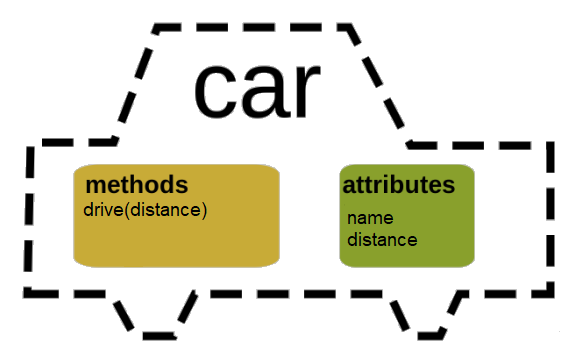
\includegraphics[width=.45\linewidth]{Car.png}
    \caption{Bauplan eines Autos -  Klasse Car}
    \label{fig:Car}
  \end{figure}

  Wir definieren dazu die folgende Klasse:

  \begin{figure}[h]
    \lstinputlisting[style=Java]{codes/Car.java}
    \caption{Bauplan eines Autos in Java - Klasse Car}
    \label{fig:Car_Java}
  \end{figure}

  \clearpage

  Wir können den Bauplan, den wir in der Abbildung \ref{fig:Car} gesehen haben in dem Java-Code
  erkennen. Ein Auto hat einen Namen und die gefahrene Distanz als Attribut. Dabei wird der Name
  als Zeichenkette, d.h. \inlinejava{String}, abgespeichert und die gefahrene Distanz als
  Gleitkommazahl, d.h. \inlinejava{double}. Des Weiteren kann ein Auto eine Strecke von einer
  vorgegebenen Distanz mit der Methode \inlinejava{drive} fahren. Mithilfe von der Klasse
  \inlinejava{Car} können wir nun verschiedene Instanzen davon erstellen.
  \index{String}

  \begin{figure}[h]
    \centering
    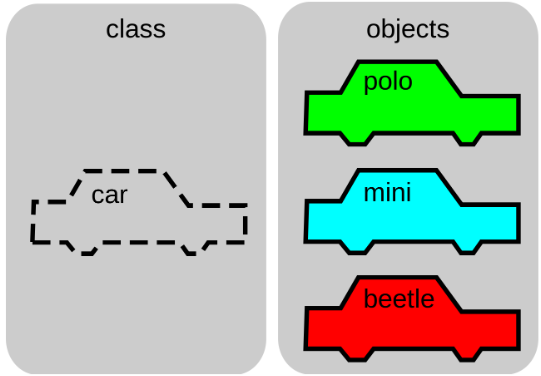
\includegraphics[width=.55\linewidth]{Car_Instances.png}
    \caption{Verschiedene Instanzen der Klasse Car}
    \label{fig:Car_Instances}
  \end{figure}
  \index{Instanzen}

  \begin{note}[title=Information:]
    Wir haben hier auch zum ersten Mal den Konstruktor einer Klasse kennen gelernt (mehr dazu bei
    \ref{sec:Konstruktor}). Wenn ein Objekt einer Klasse erstellt wird, wird zuallererst der
    Konstruktor der Klasse aufgerufen. Bei diesem Beispiel ist es dadurch möglich dem Auto einen
    Namen zu geben, der im Attribut \inlinejava{name} gespeichert wird. Man kann Objekte einer
    Klasse mit dem Schlüsselwort \inlinejava{new} instanziieren. Dann kann man auf die Attribute
    und Methoden des Objekts zugreifen.
  \end{note}
  \index{Instanziierung}
  \index{new}

  \clearpage

  \subsection{Zugriffsmodifikatoren}
  \label{sec:Zugriff}
  \index{Zugriffsmodifikatoren}
  \index{Modifier}
  \index{Attribute}
  \index{Methoden}
  \index{Klassen}
  \index{public}
  \index{protected}
  \index{package-private}
  \index{private}
  Bevor wir zu den Definitionen von \enquote{Attributen} und \enquote{Methoden} übergehen, müssen
  wir zuvor noch einen wichtigen Begriff einführen - \enquote{Zugriffsmodifikatoren} (oder
  Modifier). Zugriffsmodifikatoren bestimmen für eine gegebene Klasse, ob andere Klassen ein
  bestimmtes Attribut verwenden oder bestimmte Methoden aufrufen können. Konkret können
  Zugriffsmodifikatoren also die Sichtbarkeit von Klassen, Attributen oder Methoden einschränken.
  Dabei können zwei Ebenen unterschieden werden und je nachdem um welche Ebene es sich handelt,
  dürfen nur bestimmte Zugriffsmodifikatoren verwendet werden:

  \begin{itemize}
    \item High-Level:
    \begin{itemize}
      \item \inlinejava{public}
      \item Package-privat (kein expliziter Modifikator)
    \end{itemize}
    \item Member-Level:
    \begin{itemize}
      \item \inlinejava{public}
      \item \inlinejava{protected}
      \item Package-privat (kein expliziter Modifikator)
      \item \inlinejava{private}
    \end{itemize}
  \end{itemize}

  Mit High-Level sind Klassen, Interfaces oder Enums gemeint, die dem Dateinamen entsprechen.
  Alles Andere, wie beispielsweise Attribute oder innere Klassen gehören zum Member-Level.
  \index{Klassen}
  \index{Interface}
  \index{Enum}

  In der Tabelle \ref{tab:Zugriffsebenen} können Sie die Sichtbarkeit bezogen auf die jeweiligen
  Modifikatoren herauslesen.
  \index{Zugriffsebenen}

  \begin{table}[h]
  	\rowcolors{2}{white}{gray!25}
    \centering
    \begin{tabular}{ccccc}
      \toprule
      \textbf{Modifikator}
      & \textbf{Klasse}
      & \textbf{Package}
      & \textbf{Subklassen}
      & \textbf{Welt}
      \\
      \midrule
      \inlinejava{public} & Ja & Ja & Ja & Ja
      \\
      \inlinejava{protected} & Ja & Ja & Ja & Nein
      \\
      Kein Modifikator\footnotemark & Ja & Nein & Nein & Nein
      \\
      \inlinejava{private} & Ja & Nein & Nein & Nein
      \\
      \bottomrule
    \end{tabular}
    \caption{Zugriffsebenen}
    \label{tab:Zugriffsebenen}
  \end{table}

  \begin{itemize}
    \item Klasse: Diese Spalte gibt an, ob die Klasse selbst Zugriff auf ein Element mit dem
    entsprechenenden Modifikator hat. Wir können sehen, dass eine Klasse unabhängig vom
    Modifikator immer Zugriff auf ihre eigenen Elemente hat.
    \item Package: Diese Spalte gibt an, ob Klassen im selben Package Zugriff auf ein Element mit
    dem entsprechenenden Modifikator haben.
    \item Subklassen: Diese Spalte gibt an, ob Subklassen (Unterklassen), die außerhalb des
    Package definiert wurden, Zugriff auf ein Element mit dem entsprechenenden Modifikator haben.
    \item Welt: Diese Spalte gibt an, ob alle Klassen, unabhängig von ihrem Speicherort, Zugriff
    auf ein Element mit dem entsprechenenden Modifikator haben.
  \end{itemize}

  \begin{note}[title=Information:]
    \index{Package}
    \enquote{Ein Package ist ein Namespace mithilfe dessen eine Reihe verwandter Klassen und
    Interfaces organsisiert werden können.}
    (\url{https://docs.oracle.com/javase/tutorial/java/concepts/package.html})

    \br

    Ein Beispiel für ein Package ist \inlinejava{java.awt}. Dieses Package enthält Klassen zum
    Erstellen von Benutzeroberflächen und zum Zeichnen von Grafiken und Bildern.

    \br

    Mithilfe des folgenden Verweises können Sie sich einen Überblick über Packages verschaffen:

    \begin{center}
      \url{https://docs.oracle.com/en/java/javase/11/docs/api/allpackages-index.html}
    \end{center}

    Genaueres zu Subklassen wird im Abschnitt \ref{sec:Vererbung} und Referenzen im Abschnitt
    \ref{sec:Primitiv_Referenz_Typen} erläutert.
  \end{note}

  \footnotetext{wird auch als package-private bezeichnet}

  \clearpage

  Um zu verdeutlichen, wie genau Zugriffsmodifikatoren funktionieren, nehmen wir den
  Codeabschnitt der Abbildung \ref{fig:Car_Java} als Beispiel. Wie wir bereits gesehen haben,
  darf auf dem High-Level der Zugriffsmodifikator nur package-private oder \inlinejava{public}
  sein. Unsere Klasse soll von überall her ansprechbar sein, weshalb wir sie auf
  \inlinejava{public} setzen. Als nächstes betrachten wir die Attribute und Methoden der Klasse,
  sowie ihren Konstruktor, die alle dem Member-Level entsprechen. Die Sichtbarkeit der Attribute
  der Klasse \inlinejava{Car} stellen wir auf \inlinejava{private}, damit niemand sie
  modifizieren kann. Die Methode \inlinejava{drive(distance)} und der Konstruktor hingegen,
  sollen von außen ansprechbar sein, weshalb sie auf \inlinejava{public} gesetzt werden. Als
  Resultat erhalten wir den folgenden Codeabschnitt:

  \begin{figure}[h]
    \lstinputlisting[style=Java]{codes/Car_Modifiers.java}
    \caption{Klasse Car mit Zugriffsmodifikatoren}
  \end{figure}
  \index{Car}

  \clearpage

  \subsection{Attribute}
  \label{sec:Attribute}
  \index{Attribut}
  \index{Objekt}
  \index{Klasse}
  \index{Konventionen}
  Attribute sind Merkmale oder Eigenschaften eines Objektes einer Klasse. Sie werden direkt in
  der Klasse definiert, also nicht innerhalb von Methoden. Per Konvention definiert man sie
  unmittelbar unter der Definition der Klasse.

  \begin{note}[title=Information:]
    Diese und weitere Code-Konventionen können Sie unter dem folgenden Verweis finden:

    \begin{center}
      Abschnitt 3.1.3 Class and Interface Declarations

      \br

      \url{https://www.oracle.com/java/technologies/javase/codeconventions-fileorganization.html}
    \end{center}
  \end{note}

  Durch verschiedene Schlüsselwörter lassen sich Attribute spezifizieren. Im Allgemeinen können
  sie nach folgendem Schema definiert werden:

  \begin{center}
    Zugriffsmodifikator\(^*\) \inlinejava{static}\(^*\) Datentyp Bezeichner = Wert;
  \end{center}

  Die Begriffe, die mit einem \(^*\) (Asterisk) markiert sind, sind optional.

  \br

  In den folgenden Abschnitten werden wir uns anschauen, was mit den einzelnen Begriffen in
  diesem Schema gemeint ist.

  \paragraph{Zugriffsmodifikatoren}
  \index{Zugriffsmodifikatoren}

  Zugriffsmodifikatoren ermöglichen es die Sichtbarkeit von Attributen innerhalb von Teilen des
  Programms zu regulieren. Leichter gesagt, kann man nicht auf manche Attribute zugreifen, wenn
  bestimmte Zugriffsmodifikatoren verwendet werden. Das kann beispielsweise das Programm
  schützen, da es dem Nutzer nicht ermöglicht wahllos auf Attribute zuzugreifen und deren Werte
  zu verändern.

  \br

  Es gibt vier Typen von Attributen, die sich zwei Oberbegriffen zuordnen lassen:

  \begin{itemize}
    \item Klassenattribute
    \item Objektattribute
  \end{itemize}
  \index{Klassenattribute}
  \index{Objektattribute}

  Im folgenden wollen wir mithilfe von zwei Codeabschnitten die Verwendung von den zwei Typen von
  Attributen veranschaulichen.

  \br

  Die Klasse \inlinejava{Circle} modelliert einen Kreis. Als Attribut hat der Kreis einen Radius
  und mittels der Methoden können wir den Radius des Kreises abfragen und den Umfang und
  Flächeninhalt des Kreises bestimmen.
  \index{Circle}
  \index{Kreis}

  \begin{figure}[h]
    \centering
    \lstinputlisting[style=Java]{codes/Circle.java}
    \caption{Klasse Circle}
    \label{fig:Circle}
  \end{figure}

  \clearpage

  Die Klasse \inlinejava{Student} modelliert eine/n Studenten/in. Als Attribut hat Student eine
  Identifikationsnummer und einen Namen. Mittels der Methoden können wir die ID und den Namen des
  Student auslesen und den Namen des/r Student/in modifizieren.

  \begin{figure}[h]
    \centering
    \lstinputlisting[style=Java]{codes/Student.java}
    \caption{Klasse Student}
    \label{fig:Student}
  \end{figure}
  \index{Student}

  \paragraph{Klassenattribute}
  \index{Klassenattribute}
  \index{static}

  Klassenattribute bzw. statische Attribute sind Eigenschaften, die nicht einzelnen Objekten,
  sondern deren gesamter Klasse zugeordnet werden. Sie werden mit dem Schlüsselwort
  \inlinejava{static} gekennzeichnet. Jede Instanz der Klasse enthält die gleichen
  Klassenattribute d.h. alle Objekte der Klasse teilen sich die Klassenattribute.

  \br

  Auf Klassenattribute kann folgendermaßen zugegriffen werden:

  \begin{center}
    Klassenname.Klassenattribut
  \end{center}

  In der Abbildung \ref{fig:Circle} sehen wir jeweils den Zugriff auf das Klassenattribut
  \inlinejava{PI}. Im Allgemeinen kann der Zugriff auf Klassenattribute in der eigenen Klasse
  oder bei Subklassen auch ohne den Klassennamen erfolgen (siehe dazu Abbildung \ref{fig:Student}
  - \inlinejava{id} ; Achtung: Hierbei ist \inlinejava{id} und nicht \inlinejava{id} gemeint!).
  \index{Circle}
  \index{Student}

  \clearpage

  Außerdem gibt es noch Klassenkonstanten, die mit dem Schlüsselwort \inlinejava{final}
  gekennzeichnet werden. Wie der Name Konstante schon sagt, muss der Wert einer Konstanten
  konstant bleiben, d.h. Konstanten müssen initialisiert werden und eine erneute Zuweisung des
  gleichen oder eines anderen Wertes ist nicht möglich. Klassenkonstanten können deklarieren und
  anschließend in einem Static-Block initialisiert werden und müssen deshalb nicht sofort bei der
  Deklaration initialisiert werden.

  \begin{figure}[h]
    \centering
    \lstinputlisting[style=Java]{codes/PI_Static-Block.java}
    \caption{Initialisierung von Klassenkonstanten mittels eines Static-Blocks}
  \end{figure}

  \begin{note}[title=Information:]
    \index{Initialisierung}
    Unter Zuweisung versteht man, dass in einer Variablen ein Wert gespeichert wird. Dabei wird
    der Name einer Variablen gefolgt von einem \inlinejava{=} und dann dem Wert, den wir da rein
    speichern wollen, aufgeschrieben. Natürlich muss der zu speichernde Wert dem Datentyp
    entsprechen, den die Variable hat. Als Beispiel, wenn wir eine \inlinejava{int}-Variable
    namens \inlinejava{i} haben und dort den Wert \(15\) speichern wollen:

    \br

    \begin{center}
      \inlinejava{i = 15;}
    \end{center}

    \br

    Unter Deklarierung einer Variablen versteht man die Erstellung einer Variablen. Dabei wird
    der Datentyp der Variable gefolgt vom Variablennamen aufgeschrieben. Angenommen, wir wollen
    eine \inlinejava{int}-Variable namens \inlinejava{i} deklarieren, würden wir den folgenden
    Code schreiben:

    \br

    \begin{center}
      \inlinejava{int i;}
    \end{center}

    \br

    Unter Deklarierung und Initialisierung einer Variablen versteht man, dass die Variable sofort
    bei der Deklarierung einen Wert zugewiesen bekommen. Dabei wird der Datentyp der Variablen,
    gefolgt vom Variablennamen und einem \inlinejava{=} sowie dem Wert, der gespeichert werden
    soll und zum Datentyp passt, aufgeschrieben. Als Beispiel wollen wir die
    \inlinejava{int}-Variable namens \inlinejava{i} mit dem Wert \(15\) initialisieren:

    \br

    \begin{center}
      \inlinejava{int i = 15;}
    \end{center}
  \end{note}
  \index{Zuweisung}
  \index{Initialisierung}
  \index{Deklarierung}
  \index{Klassenkonstante}
  \index{Static-Block}

  \clearpage

  \paragraph{Objektattribute}
  \index{Objektattribute}

  Objektattribute enthalten das Schlüsselwort \inlinejava{static} nicht und gelten unabhängig
  voneinander für jede Instanz, d.h. dass jede Instanz ihre eigenen Objektattribute mit eigenen
  Werten hat. Objektattribute können nur durch ein Objekt angesprochen werden:

  \begin{center}
    Objekt.Objektattribut
  \end{center}

  In der Abbildung \ref{fig:Student} wären also folgende Attribute Objektattribute:
  \index{Student}

  \begin{itemize}
    \item \inlinejava{private final long id}: Die Identifikationsnummer des Student.
    \item \inlinejava{private String name}: Der Name des Student.
  \end{itemize}

  Jede Instanz eines \inlinejava{Student} hat seine eigene \inlinejava{id} und \inlinejava{name}.

  \br

  Betrachten wir den folgenden Codeabschnitt:

  \begin{figure}[h]
    \centering
    \lstinputlisting[style=Java]{codes/Student_Example.java}
    \caption{Beispielinstanzen der Klasse Student}
  \end{figure}

  Das Objekt \inlinejava{s1} hat somit seine eigene \inlinejava{id} (= 0) und \inlinejava{name}
  (= Max) und \inlinejava{s2} hingegen \inlinejava{id} (= 1) und \inlinejava{name} (= Erika).

  \br

  Es gibt analog zu Klassenkonstanten auch Objektkonstanten, die mit dem Schlüsselwort
  \inlinejava{final} gekennzeichnet werden. Objektkonstanten müssen ebenfalls initialisiert
  werden und eine erneute Zuweisung mit demselben oder einem anderen Wert ist nicht möglich. Es
  gibt hier auch die Möglichkeit Objektkonstanten nur zu deklarieren und anschließend in einem
  Konstruktor zu initialisieren statt sie sofort bei der Deklaration zu initialisieren.
  \index{Objektkonstanten}

  \br

  \paragraph{Standardwerte}
  \index{Standardwerte}
  \index{Referenztyp}

  Attribute (nicht Konstanten!) denen kein expliziter Wert zugewiesen wurde, nehmen automatisch
  abhängig von ihrem Datentyp einen bestimmten Standardwert an.

  \begin{table}[h]
  	\rowcolors{2}{white}{gray!25}
    \centering
    \begin{tabular}{ll}
      \toprule
      \textbf{Datentyp} & Standardwert
      \\
      \midrule
      \inlinejava{boolean} & \inlinejava{false}
      \\
      \inlinejava{byte} & \inlinejava{0}
      \\
      \inlinejava{short} & \inlinejava{0}
      \\
      \inlinejava{int} & \inlinejava{0}
      \\
      \inlinejava{long} & \inlinejava{0L}
      \\
      \inlinejava{float} & \inlinejava{0.0f}
      \\
      \inlinejava{double} & \inlinejava{0.0d}
      \\
      \inlinejava{char} & \texttt{\textcolor{stringcolor}{'\textbackslash u0000} }
      \\
      Referenztypen & \inlinejava{null}
      \\
      \bottomrule
    \end{tabular}
    \caption{Standardwerte für Attribute}
  \end{table}
  \index{boolean}
  \index{byte}
  \index{short}
  \index{int}
  \index{long}
  \index{float}
  \index{double}
  \index{char}
  \index{String}
  \index{Referenztypen}

  \begin{note}[title=Achtung:, color=tuda-orange]
    Die Standardwerte gelten nur für Attribute! Wenn Sie lokale Variablen innerhalb von Methoden
    erstellen, müssen Sie darauf achten den Variablen immer Werte zuzuweisen. Es wird zu einem
    Kompilierfehler führen, wenn Sie versuchen lokale Variablen zu verwenden, die nur deklariert
    und nicht initialisiert wurden.

    \br

    Mehr Informationen zu lokalen Variablen finden Sie im Abschnitt
    \ref{sec:Attribute_vs_lokale_Variablen_und_Konstanten}.
  \end{note}
  \index{Lokale Variablen}

  \clearpage

  \subsection{Methoden}
  \label{sec:Methoden}
  \index{Methoden}
  \index{Objekt}

  Methoden definieren das Verhalten eines Objektes, d.h. sie entsprechen Anweisungen. Sie werden
  direkt in der Klasse, typischerweise unmittelbar unter der Definition von Konstruktoren,
  definiert (Konvention, siehe Abschnitt \ref{sec:Attribute}).

  \br

  Durch verschiedene Schlüsselwörter lassen sich Methoden spezifizieren. Im Allgemeinen können
  sie nach folgendem Schema definiert werden:

  \begin{center}
    Zugriffsmodifikator\(^*\) \inlinejava{static}\(^*\) Rückgabetyp Bezeichner(Parameter\(^*\));
  \end{center}
  \index{Parameter}
  \index{Rückgabetyp}

  Die Begriffe, die mit einem \(^*\) (Asterisk) markiert sind, sind optional und Parameter werden
  auch als Argumente bezeichnet.

  \br

  In den folgenden Abschnitten werden wir uns anschauen, was mit den einzelnen Begriffen in
  diesem Schema gemeint ist.

  \br

  Falls die Methode nichts zurück liefern soll, wird das Schlüsselwort \inlinejava{void} als
  Rückgabetyp verwendet. Eine Methode kann \(n\)-beliebige Parameter haben, wobei
  \(n \in \mathbb{N}_0\)\footnote{\(\mathbb{N}_0 = \mathbb{N} \cup \{0\}\)}.
  \index{Natürliche Zahlen}
  \index{\(\mathbb{N}\)}
  \index{void}
  \index{Rückgabetyp}

  \br

  Es gibt zwei Arten von Methoden:

  \begin{itemize}
    \item Klassenmethoden
    \item Objektmethoden
  \end{itemize}
  \index{Klassenmethoden}
  \index{Objektmethode}

  \paragraph{Klassenmethoden}
  \index{Klassenmethoden}

  Klassenmethoden bzw. statische Methoden sind Verhalten, die nicht einzelnen Objekten, sondern
  deren gesamter Klasse zugeordnet werden. Sie werden mit dem Schlüsselwort \inlinejava{static}
  gekennzeichnet und können weder auf Objektattribute zugreifen noch Objektmethoden aufrufen,
  sondern nur Klassenattribute und Klassenmethoden verwenden.
  \index{Klassenattribute}

  \br

  Auf Klassenattribute kann folgendermaßen zugegriffen werden:

  \begin{center}
    Klassenname.Klassenmethode
  \end{center}

  Als Beispiel nehmen wir wieder den Codeausschnitt aus der Abbildung \ref{fig:Circle}. Wir
  erweitern die Klasse um eine Methode, die mehrere Kreise übergeben bekommt und die Summe der
  Umfänge aller Kreise zurück gibt. Da diese Methode kein Verhalten eines einzelnen Objektes
  darstellen soll, definieren wir sie als Klassenmethode.

  \begin{figure}[h]
    \centering
    \lstinputlisting[style=Java]{codes/Circle_Circumfences.java}
    \caption{Beispiel einer Klassenmethode - Klasse Circle}
    \label{fig:Circle_Circumfences}
  \end{figure}
  \index{Circle}

  Wir können nun die Klassenmethode folgendermaßen aufrufen:

  \begin{figure}[h]
    \centering
    \lstinputlisting[style=Java]{codes/Circle_Circumfences_Example.java}
    \caption{Beispielaufruf Klassenmethode - Klasse Circle}
    \label{fig:Circle_Circumfences_Example}
  \end{figure}

  Die Summe der Umfänge der Kreise in der Abbildung \ref{fig:Circle_Circumfences_Example} beträgt
  \(57.17698629533423\).


  \begin{note}[title=Information:]
    \index{Array}
    Das Codebeispiel aus der Abbildung \ref{fig:Circle_Circumfences} verwendet als Parameter
    Arrays. Genaueres zu Arrays wird im Abschnitt \ref{sec:Arrays} erläutert.
  \end{note}

  \paragraph{Objektmethoden}
  \index{Objektmethoden}

  Objektmethoden enthalten das Schlüsselwort \inlinejava{static} nicht und sind an die jeweilige
  Instanz gebunden, zu der sie gehören, d.h. dass jede Instanz andere Verhaltensweisen bei dem
  Aufruf der gleichen Methode aufweisen kann. Objektattribute können auf Klassenattribute,
  Klassenmethoden, Objektattribute und Objektmethoden zugreifen. Sie können nur mit Hilfe eines
  Objekts angesprochen werden:
  \index{Objektattribute}
  \index{Klassenattribute}
  \index{Klassenmethoden}

  \begin{center}
    Objekt.Objektmethode
  \end{center}

  Im Codeabschnitt der Abbildung \ref{fig:Circle} wären folgende Methoden Objektmethoden:
  \index{Circle}

  \begin{itemize}
    \item \inlinejava{public double getRadius()}: Gibt den Radius des Kreises wieder.
    \item \inlinejava{public double getCircumference()}: Gibt den Umfang des Kreises wieder.
    \item \inlinejava{public double getArea()}: Gibt den Flächeninhalt des Kreises wieder.
  \end{itemize}

  Sie können mit Hilfe eines Objekts aufgerufen werden:
  \index{Objekt}

  \begin{figure}[h]
    \centering
    \lstinputlisting[style=Java]{codes/Circle_Objectmethods.java}
    \caption{Beispielaufruf Objektmethoden - Klasse Circle}
  \end{figure}

  \paragraph{Überladen von Methoden}
  \label{par:ueberladen}
  \index{Überladen von Methoden}
  \index{Methodensignatur}
  \index{Parameter}
  \index{Rückgabetyp}

  Methoden lassen sich überladen, indem mindestens zwei Methoden vom gleichem Namen innerhalb
  einer Klasse definiert werden. Der Rückgabetyp und die Parameter können verschieden sein, aber
  die Parameterlisten müssen verschieden sein. Da eine Methode nicht ausschließlich durch ihren
  Namen identifiziert wird, sondern auch über die Typen, die Anzahl und die Reihenfolge ihrer
  Argumente (Parameter) - ihre Signatur, können mehrere Methoden mit demselben Namen in einer
  Klasse vorhanden sein solange sich die Signaturen unterscheiden.

  \br

  Um diesen Sachverhalt zu illustrieren können wir zusätzlich zu der Klassenmethode zur
  Bestimmung der Summen der Umfänge der Kreise in der Abbildung \ref{fig:Circle_Circumfences}
  eine ähnliche Berechnung definieren:

  \begin{figure}[h]
    \centering
    \lstinputlisting[style=Java]{codes/Circle_Circumfences_Overloading.java}
    \caption{Überladen von Methoden - Klasse Circle}
  \end{figure}
  \index{Circle}

  Wir können nun statt ein \inlinejava{Circle[]} zu erstellen nur die Radien als
  \inlinejava{double[]} zur Berechnung der Umfänge der Kreise übergeben. Diese Methode
  unterscheidet sich von der Signatur her von der zuvor definierten Methode, da sich die
  Parameter der beiden Methoden unterscheiden (\inlinejava{Circle[]} \(\neq\) \inlinejava{double[]}).

  \br

  Beim Aufruf der Methode wird dann, je nach eingegebenen Parametern, die Methode genommen, die
  zu den Parametern passt. Der Vorteil vom Überladen einer Methode ist, dass man mehrere Methoden
  mit der gleichen Funktionalität erstellen kann, die für verschiedene Zwecke genutzt werden
  können. Wie hier zu sehen ist, haben beide \inlinejava{getCircumferences}-Methoden die gleiche
  Funktionalität. Aber einmal kann man als Eingabe Kreise übergeben und ebenfalls nur die Radien.
  Je nach Anwendungsfall kann also die passende Methode gewählt werden.

  \paragraph{Getter und Setter}
  \index{Getter}
  \index{Setter}

  Im Zusammenhang zu Methoden sollte man auch als Spezialfall die Setter und Getter-Methoden
  erwähnen. Es gilt als ein guter Programmierstil, wenn man Attribute auf \inlinejava{private}
  setzt und Getter und Setter-Methoden zum Zugriff auf die Attribute verwendet. Wie der Name
  schon sagt, soll mit der Setter-Methode der Wert eines Attributs gesetzt werden können. Mit der
  Getter-Methode wird dementsprechend der Wert eines Attributs zurückgegeben.

  \br

  Diese beiden Methoden vereinfachen den Zugriff auf die Attribute und ermöglichen es das
  Programm besser zu schützen. Wenn beispielsweise der Wert eines Attributs innerhalb von einem
  bestimmten eingegrenzten Bereich liegen soll, ist es einfacher eine Setter-Methode zu
  definieren, als überall, wo das Attribut verwendet wird, auf den Bereich zu überprüfen.
  Außerdem kann man bei Attributen, die nicht verändert werden sollen, keine Setter-Methode
  definieren und damit den Zugriff darauf regeln.

  \clearpage

  \subsection{Konstruktor}
  \label{sec:Konstruktor}
  \index{Konstruktor}
  \index{Car}
  \index{Circle}
  \index{Student}
  \index{Klasse}
  \index{new}

  Wir haben bereits Konstruktoren in verschiedenen Beispielen, wie in den Abbildungen
  \ref{fig:Car}, \ref{fig:Circle} und \ref{fig:Student}, gesehen. In diesem Abschnitt wollen wir
  uns genauer damit befassen, was man genau unter einem Konstruktor versteht.

  \br

  Ein Konstruktor hat keinen Rückgabewert und sein Name ist gleich dem Namen der Klasse.
  Konstruktoren werden nur einmal aufgerufen und zwar, wenn man ein neues Objekt erstellt. Man
  kann neue Objekte einer Klasse mit dem Schlüsselwort \inlinejava{new} instanziieren.
  Beispielweise, wenn wir ein Objekt der Klasse \inlinejava{Student}, wie in der Abbildung
  \ref{fig:Student}, erstellen wollen, schreiben wir:

  \br

  \begin{center}
    \inlinejava{Student student = new Student("Max");}
  \end{center}

  \br

  In die runden Klammern nach dem Namen der Klasse (hier: \inlinejava{Student}), kommen die Werte
  für die Parameter des Konstruktors. Da der Konstruktor von \inlinejava{Student} den Parameter
  \inlinejava{name} hat, kommt dort ein Wert, der einen Namen repräsentieren soll, hin.

  \begin{note}[title=Achtung:, color=tuda-orange]
    Beim Aufrufen und Zuweisen wird die dann die Adresse des entsprechenden erstellten Objekts
    zurückgegeben und nicht das Objekt selbst (siehe dazu auch \ref{sec:Referenztypen} und
    \ref{sec:Vergleich_Refernztypen_primitive_Datentypen}).
  \end{note}

  \br

  Konstruktoren werden nicht vererbt und, wenn eine Klasse keinen Konstruktor hat, wird vom
  Compiler automatisch der leere Konstruktor (no-args constructor - keine Argumente Konstruktor)
  aufgerufen.

  \br

  Im Konstruktor können Anweisungen definiert werden, die während der Erstellung eines Objektes
  gebraucht werden. Beispielsweise können dabei Attributen initialisiert oder bestimmte Methoden
  angesprochen werden (siehe dazu Abbildung \ref{fig:Student}).

  \br

  Innerhalb von einem Konstruktor werden oft die Schlüsselwörter \inlinejava{this} und
  \inlinejava{super} verwendet.

  \br

  Das Schlüsselwort \inlinejava{this} spricht das aktuelle Objekt an, d.h. wir können mit diesem
  Schlüsselwort auf die aktuellen Attribute und Methoden des Objektes zugreifen. Wenn ein
  gleichnamige/r Parameter oder lokale Variable vorhanden ist, kann mithilfe von diesem
  Schlüsselwort das Attribut von diesem/r Parameter oder lokalen Variable unterschieden werden.
  Als Beispiel haben wir in der Klasse \inlinejava{Student} gesehen, dass der Konstruktor einen
  Parameter enthält, wessen Name mit einem Attribut der Klasse übereinstimmt. Um zu
  unterscheiden, ob das Attribut oder der Parameter angesprochen werden soll, kann das
  Schlüsselwort \inlinejava{this} verwendet werden.
  \index{this}

  \br

  Wir können zum Codebeispiel \inlinejava{Student} (Abbildung \ref{fig:Student}) das
  Schlüsselwort \inlinejava{this} an den entsprechenden Stellen hinzufügen und erhalten den
  folgenden Code:
  \index{Student}

  \begin{figure}[h]
    \centering
    \lstinputlisting[style=Java]{codes/Student_this.java}
    \caption{Verwendung von this - Klasse Student}
  \end{figure}

  Das Schlüsselwort \inlinejava{super} spricht die Oberklasse an, d.h. die Klasse von der die
  jetzige Klasse abgeleitet ist (genaueres dazu wird im Abschnitt \ref{sec:Vererbung} erläutert).
  Durch dieses Schlüsselwort können wir den Konstruktor der Oberklasse aufrufen und Attribute und
  Methoden der Oberklasse ansprechen. Falls der Konstruktor der Oberklasse aufgerufen werden
  soll, muss es als erste Anweisung im abgeleiteten Konstruktor geschehen. Falls kein Konstruktor
  der Oberklasse aufgerufen wird, wird der Compiler den Standardkonstruktor der Oberklasse
  aufrufen, falls einer definiert ist.
  \index{super}

  \clearpage


  \section{Vererbung}
  \label{sec:Vererbung}
  \index{Vererbung}
  \index{Objektorientierung}
  \index{Hierarchie}
  \index{Klassen}

  Die Vererbung ist ein grundlegendes Konzept der Objektorientierung, mit welcher Hierarchien in
  der realen Welt mit Hilfe von Klassen modelliert werden können. Beispielsweise können damit die
  hierarchischen Beziehungen zwischen Klassen dargestellt werden.

  \br

  Die Basisklasse stellt eine Verallgemeinerung eines Objekt (\textit{Generalisierung}) mit
  seinem Verhalten dar, die durch die abgeleitete Klassen spezifiziert werden kann. Innerhalb der
  abgeleiteten Klassen können also eigene Ausprägungen und ein eigenes Verhalten
  (\textit{Spezialisierung}) entstehen, wobei die Grundzüge von der Basisklasse vererbt wurden.
  \index{Generalisierung}
  \index{Spezialisierung}

  \br

  Java unterstützt nur Einfachvererbungen und Vererbungen werden mit dem Schlüsselwort
  \inlinejava{extends} nach dem Klassennamen gekennzeichnet gefolgt von der Klasse, welche die
  Klasse erweitern soll.
  \index{Einfachvererbungen}

  \begin{figure}[h]
    \centering
    \begin{minipage}[t]{.425\linewidth}
      \lstinputlisting[style=Java]{codes/Base_Class.java}
    \end{minipage}
    \hfill\vline\hfill
    \begin{minipage}[t]{.55\linewidth}
      \lstinputlisting[style=Java]{codes/Derived_Class.java}
    \end{minipage}
    \caption{Formaler Aufbau}
  \end{figure}

  \begin{figure}[h]
    \centering
    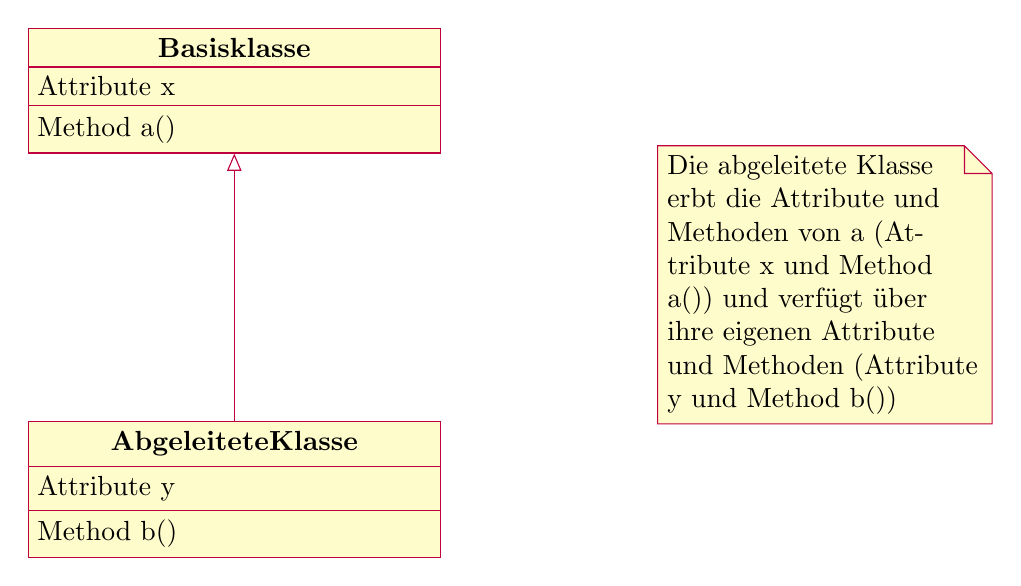
\begin{tikzpicture}
      % Class: Superclass
      \begin{class}[text width=5cm]{Basisklasse}{0,0}
        \attribute{Attribute x}
        \operation{Method a()}
      \end{class}

      % Class: Subclass
      \begin{class}[text width=5cm]{AbgeleiteteKlasse}{0,-5}
        \inherit{Basisklasse}
        \attribute{Attribute y}
        \operation{Method b()}
      \end{class}

      % Note
      \umlnote (note) at  (7.5,-1.5) {Die abgeleitete Klasse erbt die Attribute und Methoden von
      a (Attribute x und Method a()) und verfügt über ihre eigenen Attribute und Methoden
      (Attribute y und Method b())};
    \end{tikzpicture}
    \caption{Darstellung des formalen Aufbaus im UML-Diagramm}
  \end{figure}
  \index{UML}

  Durch eine abstrakte Modellierung kann in der objektorientierten Programmierung, vor allem auf
  höheren und komplexeren Abstraktionsebenen, eine bessere Strukturierung ermöglicht werden.
  Dadurch wird es leichter eine weniger fehleranfällige Abbildung der realen Welt zu erschaffen.
  \index{Abstrakte Modellierung}
  \index{Objektorientierten Programmierung}
  \br

  Eine wichtige Eigenschaft der Vererbung ist die \textit{Erweiterbarkeit}. Die Modellierung von
  Abstraktionsebenen ermöglicht es uns bestimmte Strukturen der Klasse wiederzuverwenden und
  vermeidet die \textit{Redundanz} von gleichen oder ähnlichen Codeabschnitten, die ansonsten
  mehrfach geschrieben werden müssten. Dadurch wird ebenfalls die \textit{Fehleranfälligkeit}
  reduziert.
  \index{Erweiterbarkeit}
  \index{Redundanz}
  \index{Fehleranfälligkeit}

  \clearpage

  Im folgenden machen wir wieder ein Beispiel: Wir würden gerne Vögel modellieren. Dafür
  definieren wir als Basisklasse die Klasse \inlinejava{Bird}. Daraus können wir verschiedene
  Arten von Vögeln ableiten, die gemeinsame Verhalten und Eigenschaften aufweisen.
  \index{Vogel}
  \index{Bird}

  \begin{figure}[h]
    \centering
    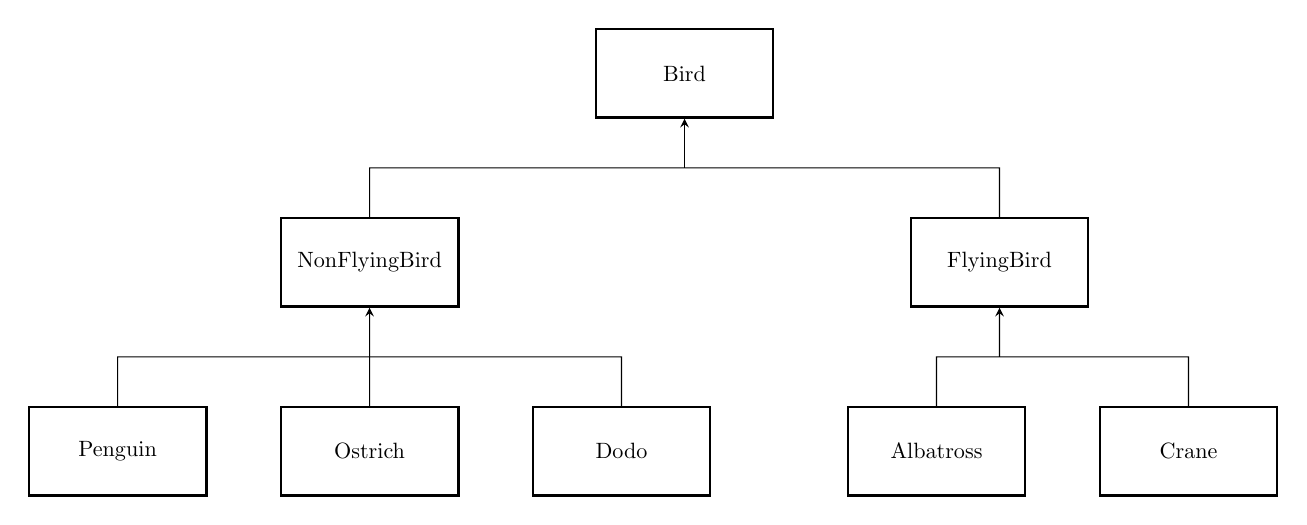
\begin{tikzpicture}[scale=.8, transform shape]
      \begin{scope}[
        every node/.style={
        draw,
        line width=1pt,
        minimum height=40pt,
        minimum width=80pt,
        transform shape,
        shape=rectangle,
        }
      ]
        \node (a) at (0, 0) {Bird};
        \node (b) at (-5, -3) {NonFlyingBird};
        \node (c) at (5, -3) {FlyingBird};
        \node (d) at (-9, -6) {Penguin};
        \node (e) at (-5, -6) {Ostrich};
        \node (g) at (-1, -6) {Dodo};
        \node (h) at (4, -6) {Albatross};
        \node (i) at (8, -6) {Crane};

        \draw[-stealth] (0, -1.5) -- (a);
        \draw (b.north) -- (-5, -1.5) -- (0, -1.5);
        \draw (c.north) -- (5, -1.5) -- (0, -1.5);

        \draw[-stealth] (e) -- (b);
        \draw (d.north) -- (-9, -4.5) -- (-5, -4.5);
        \draw (g.north) -- (-1, -4.5) -- (-5, -4.5);

        \draw[-stealth] (5, -4.5) -- (c);
        \draw (h.north) -- (4, -4.5) -- (5, -4.5);
        \draw (i.north) -- (8, -4.5) -- (5, -4.5);
      \end{scope}
    \end{tikzpicture}
    \caption{Typhierarchie - Modellierung von Vögeln}
    \label{fig:Type_hierarchy_Bird}
  \end{figure}

  Wir würden also in der Klasse \inlinejava{Bird} alle Verhaltensweisen und Eigenschaften
  definieren, die alle Vögel gemeinsam haben. In der Klasse \inlinejava{NonFlyingBird} würden wir
  alle Eigenschaften und Verhaltensweisen definieren, die alle Vögel, die nicht fliegen können,
  gemeinsam haben usw.
  \index{NonFlyingBird}

  \br

  Dadurch ist es uns möglich Wiederholungen und Fehler zu vermeiden. Wir würden nämlich
  beispielsweise die Methode, die das Fliegen darstellen soll, nicht in \inlinejava{Bird} und
  \inlinejava{NonFlyingBird} definieren, sondern in \inlinejava{FlyingBird}. Dadurch würden wir
  sicher stellen, dass einerseits Vögel, wie \inlinejava{Penguin}, nicht auf die Methode
  zugreifen können. Andererseits müssen wir auch nicht die Methode bei jeder Vogelart neu
  definieren und Vögel, wie \inlinejava{Crane}, hätten automatisch Zugriff darauf, weil sie von
  \inlinejava{FlyingBird} abgeleitet sind.
  \index{FlyingBird}

  \subsection{Subtypen}
  \label{sec:Subtypen}
  \index{Subtypen}
  Als Subtypen einer Klasse bezeichnet man

  \begin{itemize}
    \item die Klassen, die entweder direkt \inlinejava{extends} oder indirekt von einer Klasse
    abgeleitet sind.
    \item bei einem Interface die Interfaces, die es direkt oder indirekt erweitern, und die
    Klassen, die es oder eins der erweiterten Interfaces direkt oder indirekt implementieren.
    \item bei einem Array die Komponententypen, bei denen der Typ ein Subtyp ist (Erklärung zu
    Arrays siehe \ref{sec:Arrays})
  \end{itemize}
  \index{extends}
  \index{Arrays}

  Das Gegenstück zu Subtyp ist der Supertyp.
  \index{Supertyp}

  \paragraph{Statischer und dynamischer Typ}
  \label{par:Statischer_und_dynamischer_Typ}
  \index{Statischer Typ}
  \index{Dynamischer Typ}

  Der statische Typ ist der Typ, der bei der Variablendeklaration angegeben wird. Er ist bei der
  Kompilierung schon bekannt.

  \br

  Der dynamische Typ ist der Typ des tatsächlichen Objekts, der erst zur Laufzeit bekannt ist.
  Er kann vom statischen Typ abweichen und ist entweder gleich dem statischen Typ oder ein Subtyp
  des statischen Typs.

  \br

  Der formale Aufbau bei einer Variablendeklaration sieht also folgendermaßen aus:

  \begin{center}
  <Statischer Typ>
    Bezeichner = <Dynamischer Typ>
  \end{center}

  \clearpage
  Um sich das Ganze zu veranschaulichen, betrachten wir den folgenden Codeabschnitt:
  \index{Rectangle}
  \index{Square}

  \begin{figure}[h]
    \centering
    \lstinputlisting[style=Java]{codes/Rectangle_and_Square_1.java}
    \caption{Vererbung Klasse Rectangle}
    \label{fig:rec_overload}
  \end{figure}

  \begin{figure}[H]
    \centering
    \lstinputlisting[style=Java]{codes/Rectangle_and_Square_2.java}
    \caption{Vererbung Klasse Square}
    \label{fig:sq_overload}
  \end{figure}

  \clearpage

  Wir können daraus als Beispiel die folgenden Objekte instanziieren:
  \index{Instanziierung}

  \begin{figure}[h]
    \centering
    \lstinputlisting[style=Java]{codes/Rectangle_and_Square_Example.java}
    \caption{Vererbung Klasse Rectangle und Square}
    \label{fig:Rectangle_and_Square_Example}
  \end{figure}

  Wie wir kennen gelernt haben, kann ein Objekt mit dem statischen Typ \inlinejava{Rectangle}
  entweder \inlinejava{Rectangle} oder ein Subtyp davon als dynamischen Typ haben.

  \br

  Gehen wir das Beispiel nochmal genauer durch: In Zeile 1 und 2 entspricht der statische Typ dem
  dynamischen Typ. Aber in Zeile 4 können wir sehen, dass wir als dynamischen Typ einen Subtyp
  von \inlinejava{Rectangle} genommen haben. Hier wird der Subtyp \inlinejava{Square} der
  Referenz vom Supertyp \inlinejava{Rectangle} zugewiesen.

  \br

  Der statische Typ darüber auf welche Attribute und Methoden zugegriffen werden darf und der
  dynamische Typ welche Implementation einer Methode aufgerufen wird.
  \index{Attribute}
  \index{Methoden}
  \index{Implementation}

  \br
  \begin{note}[title=Information:]
    Ein zentraler Punkt bei Subtypen ist also, dass man beim dynamischen Typ statt der
    eigentlichen Klassen ebenfalls ihre Subtypen verwenden kann. Das gilt für die Deklaration von
    Attributen, Variablen, sowie dem Parameterwert und Rückgabetyp von Methoden.

    \br

    Beim Parameterwert wird deshalb zwischen dem aktualen Wert (der Parameterwert, der eingesetzt
    wird) und dem formalen Wert (der in der Definition des Parameters in der Methode steht)
    unterschieden.
  \end{note}

  \subsection{Überschreiben von Methoden}
  \index{Überschreiben von Methoden}
  \index{Überladen von Methoden}

  Wir unterscheiden das \emph{Überschreiben} einer Methode vom \emph{Überladen} einer Methode.
  Das Überladen einer Methode haben wir bereits in Abschnitt \ref{par:ueberladen} kennen gelernt.
  Das Überschreiben von Methoden erlaubt es einer abgeleiteten Klasse, eine eigene
  Implementierung einer von der Basisklasse geerbten Methode zu definieren. Die Unterscheidung,
  ob die ursprüngliche oder die neue Methode beim Aufruf der überschriebenen Methode verwendet
  wird, wird anhand des dynamischen Typs (genaueres dazu im Abschnitt
  \ref{par:Statischer_und_dynamischer_Typ}) des Objektes getroffen.

  \br

  Mithilfe vom Überschreiben einer Methode kann man erreichen, dass Methoden, deren
  Funktionalität in der abgeleiteten Klasse verändert werden soll, einfach überschrieben werden.
  Gleichzeitig können aber die anderen Methoden der Oberklasse immer noch weiter verwendet werden.

  \begin{note}[title=Information:]
    Es gibt also zwei Fälle bei dem Überschreiben einer Methode:

    \begin{itemize}
      \item Ist der dynamische Typ des betrachteten Objekts die abgeleitete Klasse, wird die
      Methode von der abgeleiteten Klasse verwendet.
      \item Ist er hingegen die Basisklasse, so wird die Methode von der Basisklasse verwendet.
    \end{itemize}
  \end{note}

  Zur Veranschaulichung machen wir uns wieder ein Beispiel. Wir nehmen den Code aus
  \ref{fig:rec_overload} und \ref{fig:sq_overload}. In dem Codeabschnitt \ref{fig:sq_overload}
  wurde eine Klasse \inlinejava{Square} erstellt, die von der Klasse \inlinejava{Rectangle}
  abgeleitet ist.
  \index{Square}
  \br

  Wie wir sehen können, wurde in \inlinejava{Square} nur die Methode
  \inlinejava{getCircumference} überschrieben. Würden wir ein Objekt vom statischen Typ
  \inlinejava{Rectangle} und dynamischen Typ \inlinejava{Square} haben und
  \inlinejava{getCircumference} aufrufen, würde die Methode, die in \inlinejava{Square} definiert
  wurde, aufgerufen werden. Bei einem statischen und dynamischen Typ von \inlinejava{Rectangle}
  würde die Methode \inlinejava{getCircumference} von \inlinejava{Rectangle} genommen werden.

  \br

  Überschriebene Methoden können mit der Annotation \inlinejava{@Override} versehen werden. Die
  Annotation \inlinejava{@Override} gibt an, dass die Methode der untergeordneten Klasse die
  Methode der Basisklasse überschreibt. Aus zwei Gründen ist die Annotation
  \inlinejava{@Override} nützlich:
  \index{Override}
  \index{Annotation}

  \begin{itemize}
    \item Wenn die mit der Annotation versehene Methode nichts überschreibt, gibt der Compiler
    eine Warnung aus. Dadurch können Fehler vermieden werden
    \item Es kann helfen, den Quellcode lesbarer zu machen.
  \end{itemize}

  \clearpage

  \subsection{Methodentabelle}
  \index{Methodentabelle}
  \index{Objekt}
  Wir haben bereits kennen gelernt, dass der dynamische Typ eines Objektes eine Rolle dabei
  spielt, welche Implementation einer Methode aufgerufen wird. Aber was genau versteht man unter
  \enquote{Welche Implementation einer Methode aufgerufen wird}?

  \br

  Jedes Objekt einer Klasse enthält einen Verweis auf ein anonymes Objekt mit verborgenen
  Informationen. Dieses anonyme Objekt wird einmal in einem Programm pro Klasse eingerichtet. Die
  Informationen beziehen sich auf die Klasse selbst, ihre Methoden und ihre Attribute. Außerdem
  enthält das anonyme Objekt auch die Methodentabelle.

  \br

  Im Folgenden wollen wir die Abbildung \ref{fig:Rectangle_and_Square_Example} und die
  entsprechenden Definitionen der dort verwendeten Klassen zur Veranschaulichung des Speichers
  und der Methodentabelle nutzen.

  \br

  Zuerst schauen wir an, wie die verborgenen Informationen im Speicher aussehen:
  \begin{figure}[h]
    \centering
    \begin{memory}
      \allocatedummy{5}
      \allocatedummy{15}
      \allocatedummy{25}
      \allocate{7}{8}
      \allocate{17}{19}
      \allocate{26}{27}
      \assign{5}{7}{\inlinejava{width}}
      \assign{10}{8}{\inlinejava{height}}
      \assign{25}{26}{\inlinejava{width}}
      \assign{29}{27}{\inlinejava{height}}
      \assign{18}{18}{Daten für Rectangle}
      \assignblock{7}{18}
      \assignblock{26}{18}
    \end{memory}
    \caption{Anonymes Objekt zur Klasse \inlinejava{Rectangle}}
  \end{figure}
  \index{Speicher}

  Wir sehen hier zwei Objekte von \inlinejava{Rectangle}, die jeweils die Attribute
  \inlinejava{width} und \inlinejava{height} haben. Jedes von diesen zwei Objekten hat dabei
  einen Verweis auf die verborgenen Informationen, die hier als \enquote{Daten für
  \inlinejava{Rectangle}} bezeichnet werden. Im Allgemeinen soll die Abbildung also zeigen, dass,
  wenn man ein Objekt von \inlinejava{Rectangle} erstellt, es automatisch einen Verweis auf die
  verborgenen Informationen bekommt. Jedes Objekt vom Typ \inlinejava{Rectangle} kann somit auf
  diese Informationen zugreifen. Das Beispiel lässt sich auf alle möglichen Klassen, nicht nur
  auf \inlinejava{Rectangle}, übertragen.

  \br

  Mithilfe der Methodentabelle, die zu den verborgenen Informationen gehört, kann man sehen,
  welche Implementation einer Methode für ein gegebenes Objekt verwendet wird.

  \br

  Wir wollen die Funktionsweise von der Methodentabelle anhand des gegebenen Beispiels kennen
  lernen:

  \begin{figure}[h]
    \centering
    \begin{tikzpicture}[scale=.9, transform shape]
      \begin{scope}[every node/.style={node distance=10pt}]
        \node (rectangle) at (0, 0) {rectangle};
        \node (square) at (0, -2.5){square};
        \node (rs) at (0, -5) {rs};
      \end{scope}
      \begin{scope}[
        every node/.style={
        draw,
        fill=black,
        line width=1pt,
        minimum height=30pt,
        minimum width=15pt,
        shape=rectangle,
        }
      ]
        \node (rectangle-box) at (2.5, 0) {};
        \node (square-box) at (2.5, -2.5) {};
        \node (rs-box) at (2.5, -5) {};
      \end{scope}
      \draw[->] (rectangle) -- (rectangle-box);
      \draw[->] (square) -- (square-box);
      \draw[->] (rs) -- (rs-box);
      \begin{scope}[
        every node/.style={
        draw,
        line width=1pt,
        minimum height=20pt,
        minimum width=90pt,
        node distance=-1pt,
        shape=rectangle,
        }
      ]
        \node[fill=black] (rectangle-ref) at (7.5, 1.5) {};
        \node[below=of {rectangle-ref}] (rectangle-width) {getWidth()};
        \node[below=of {rectangle-width}] (rectangle-height) {getHeight()};
        \node[below=of {rectangle-height}] (rectangle-area) {getArea()};
        \node[below=of {rectangle-area}] (rectangle-circumference) {getCircumference()};

        \node[fill=black] (square-ref) at (7.5, -3.5) {};
        \node[below=of {square-ref}] (square-width) {getWidth()};
        \node[below=of {square-width}] (square-height) {getHeight()};
        \node[below=of {square-height}] (square-area) {getArea()};
        \node[below=of {square-area}] (square-circumference) {getCircumference()};
        \node[below=of {square-circumference}] (square-diagonallength) {getDiagonalLength()};
      \end{scope}
      \draw[->] (rectangle-box.east) -- (rectangle-ref.west);
      \draw[->] (square-box.east) -- (square-ref.west);
      \draw[->] (rs-box.east) -- (square-ref.west);

      \node (width) at (14, -2) {getWidth() in Rectangle};
      \draw[->] (rectangle-width.east) -- (width);
      \draw[->] (square-width.east) -- (width);

      \node (height) at (14, -3) {getHeight() in Rectangle};
      \draw[->] (rectangle-height.east) -- (height.west);
      \draw[->] (square-height.east) -- (height);

      \node (area) at (14, -4) {getArea() in Rectangle};
      \draw[->] (rectangle-area.east) -- (area.west);
      \draw[->] (square-area.east) -- (area);

      \node (circumference-rectangle) at (14, 1) {getCircumference() in Rectangle};
      \draw[->] (rectangle-circumference.east) -- (circumference-rectangle);

      \node (circumference-square) at (14, -6) {getCircumference() in Square};
      \draw[->] (square-circumference.east) -- (circumference-square);

      \node (diagonallength-square) at (14, -7) {getDiagonalLength() in Square};
      \draw[->] (square-diagonallength.east) -- (diagonallength-square);
    \end{tikzpicture}
    \caption{Methodentabelle bezüglich des Codeabschnitt aus der Abbildung \ref{fig:Rectangle_and_Square_Example}}
  \end{figure}
  \index{Rectangle}
  \index{Square}

  \clearpage

  Wir wollen uns die einzelnen Variablen anschauen und herausfinden, welche Methoden welcher
  Klassen bei welcher Variablen aufgerufen werden.

  \begin{itemize}
    \item Objekt \inlinejava{Rectangle} hat den dynamischen und statischen Typ
    \inlinejava{Rectangle}, deshalb ist es klar, dass die Implementation \inlinejava{getWidth()},
    \inlinejava{getHeight()}, \inlinejava{getArea()} und \inlinejava{getCircumference()} von
    \inlinejava{Rectangle} verwendet werden.
    \item  Objekt \inlinejava{Square} hat den statischen und dynamischen Typ \inlinejava{Square},
    deshalb wird \inlinejava{getCircumference} und \inlinejava{getDiagonalLength()} von
    \inlinejava{Square} genommen. Die Methoden \inlinejava{getWidth()}, \inlinejava{getHeight()}
    und\inlinejava{getArea()} werden von \inlinejava{Rectangle} verwendet, da es keine
    Implementation von diesen Methoden in \inlinejava{Square} gibt.
    \item Objekt \inlinejava{rs} hat den statischen Typ \inlinejava{Rectangle} und den
    dynamischen Typ \inlinejava{Square}. Wegen dem dynamischen Typ \inlinejava{Square} wird die
    Implementation \inlinejava{getCircumference} von \inlinejava{Square} genommen, obwohl das
    Objekt den statischen Typ \inlinejava{Rectangle} hat. Natürlich wird wieder
    \inlinejava{getWidth()}, \inlinejava{getHeight()} und\inlinejava{getArea()} von
    \inlinejava{Rectangle} verwendet. Achtung: Auf die Methode \inlinejava{getDiagonalLength()}
    kann aufgrund von dem statischen Typs nicht zugegriffen werden!
  \end{itemize}

  \paragraph{Casting}
  \label{sec:Casting}
  \index{Casting}
  \index{Upcasting}
  \index{Downcasting}

  Wenn eine Variable von einem bestimmten Typ ist, aber man einen anderen Typ verwenden will, wie
  z.B. einen abgeleiteten Typ, ist es möglich die Variable auf den entsprechenden Typ zu
  \enquote{casten}.

  \br

  Casting bedeutet so etwas wie Typumwandlung und kann entweder explizit oder implizit
  durchgeführt werden. Beim impliziten Casting wird der Typ nicht angegeben, sondern die
  Typumwandlung geschieht automatisch. Implizites Casting ist immer dann möglich, wenn das
  Casting unbedenklich ist, d.h. der Typ in den anderen Typ ohne Datenverlust umgewandelt werden
  kann (bspw. \inlinejava{short} zu \inlinejava{int}). Beim expliziten Casting muss der Typ, in
  den umgewandelt werden soll, explizit angegeben werden.

  \br

  Der Vorteil und der Sinn vom Casting lässt sich an dem folgenden Beispiel zeigen: Nehmen wir an
  wir haben den statischen Typ einer Klasse \inlinejava{Rectangle} genommen, wollen aber auf die
  Methoden, die erst in der Klasse \inlinejava{Square} definiert werden, zugreifen. Das geht nur,
  wenn wir vorher die zugehörige Variable downcasten, d.h. in den Typ \inlinejava{Square}
  umwandeln. Das können wir durch explizites Casting erreichen.

  \br

  Um eine Variable explizit zu einem Typ zu casten, können wir das folgende Schema verwenden
  \begin{center}
  (Typ des Casting)
    Objekt
  \end{center}

  In unserem konkreten Beispiel würde das so aussehen, wenn wir auf die Methode
  \inlinejava{getDiagonalLength()} von \inlinejava{Square} zugreifen wollen:

  \begin{center}
    ((Square) rs).getDiagonalLength();
  \end{center}

  \clearpage


  \section{Interfaces und abstrakte Klassen}
  \label{sec:Interfaces_abstrakte_Klassen}
  \index{Interfaces}
  \index{Abstrakte Klasse}

  \subsection{Interface}
  \index{Instanziierung}
  \index{Schnittstelle}
  \index{Vertrag}
  Ein Interface ist eine Schnittstelle, die trennt, \emph{was} eine Klasse tut, und \emph{wie}
  die Klasse es tut, und in einem Interface können keine Objekte instanziiert werden.

  \br

  Das Interface stellt einen Vertrag dar: Es setzt fest, was ein Kunde erwarten kann, indem im
  Vorhinein die Funktionalitäten beschrieben werden, die erfüllt werden sollen, und genaue
  Methoden benannt werden. Der Kunde weiß damit, welche Methoden und Funktionalitäten eine
  Klasse, die das Interface implementiert, haben muss. Außerdem lässt das Interface dem
  Entwickelnden die Freiheit, wie diese Erwartung durch die eigentliche Implementierung erfüllt
  wird. Das heißt, dass die genaue Implementierung der beschriebenen Methoden durch den
  Entwickelnden in der das Interface implementierenden Klasse erfolgt und nicht direkt im
  Interface selbst ersichtlich ist. Interfaces erlauben damit die Verwendung von
  Funktionalitäten, ohne, dass die eigentliche darunterliegende Implementierung bekannt ist.

  \br

  Zur Visualisierung kann man sich Interfaces als eine Art Schablone vorstellen.
  Die Schablone gibt eine Vorlage, wie das Produkt am Ende aussehen soll. Allerdings gibt sie
  nicht alles vor, sondern ihr Inneres ist frei gestaltbar, solange die Vorgaben der Schablone
  eingehalten werden.
  \index{Schablone}

  \br

  Im Interface ist alles implizit \inlinejava{public}, weshalb der Zugriffsmodifikator in
  Interface weggelassen werden kann. Zusätzlich sind alle Methoden implizit \inlinejava{abstract}
  und das Schlüsselwort \inlinejava{abstract} sagt aus, dass die Methode nicht implementiert ist.
  Es kann hier ebenfalls weggelassen werden. Es gibt allerdings einige Ausnahmen:
  \index{public}
  \index{abstract}

  \begin{itemize}
    \index{default}
    \index{private}
    \item Seit Java 8 können Objektmethoden, welche mit dem Schlüsselwort \inlinejava{default}
    versehen sind, implementiert werden. Dadurch können die Entwickelnden den Interfaces neue
    Methoden hinzufügen ohne die Klassen zu beeinflussen, die diese Interfaces implementieren.
    \item Seit Java 9 können Methoden können mit dem Zugriffsmodifikator \inlinejava{private}
    implementiert werden. Diese privaten Methoden verbessern die Wiederverwendbarkeit von Code
    innerhalb von Schnittstellen. Das passiert dadurch, dass man Code in private Methoden
    auslagern kann, die dann von außen nicht sichtbar sind und bspw. in default-Methoden
    verwendet werden können.
  \end{itemize}

  Außerdem können in einem Interface nur Objektmethoden deklariert werden.
  \index{Objektmethoden}

  \br

  Da ein Interface zustandslos ist, können keine Objektattribute definiert werden, sondern nur
  Klassenkonstanten. Also können bei der Definition von Klassenkonstanten die Schlüsselwörter
  \inlinejava{static final} weggelassen werden, da sie sowieso implizit verwendet werden.
  \index{Objektattribute}
  \index{Klassenkonstanten}

  Eine Klasse kann ein Interface oder mehrere Interfaces mit dem Schlüsselwort
  \inlinejava{implements} (im Klassenkopf) implementieren. Falls mehrere Interfaces implementiert
  werden sollen, dann werden die Namen mit einem Komma voneinander getrennt hintereinander
  notiert. Eine Klasse muss alle nicht implementierten Methoden der implementierten Interfaces
  implementieren, sonst muss die Klasse als abstrakt gekennzeichnet werden.
  \index{implements}

  \br

  Ein Interface kann auch ein oder mehrere Interfaces erweitern. Das wird mit dem Schlüsselwort
  \inlinejava{extends} gekennzeichnet und die entsprechenden Interfaces werden mit einem Komma
  getrennt nacheinander aufgeschrieben.

  \clearpage
  Als Beispiel definieren wir uns zwei Interface:

  \begin{itemize}
    \item Das Interface \inlinejava{Swimming} bietet die Möglichkeit eine bestimmte Distanz zu
    schwimmen.
    \item Das Interface \inlinejava{Flying} bietet die Möglichkeit eine bestimmte Distanz zu
    fliegen. Außerdem beinhaltet es eine Klassenkonstante \inlinejava{SPEED}. Mithilfe von dieser
    Konstante ist es möglich festzulegen, dass einige Objekte mehr Distanz zurücklegen können,
    weil sie eine höhere Geschwindigkeit haben.
  \end{itemize}

  Jetzt können wir einen Schwan modellieren, der schwimmen und fliegen kann. Der
  Zugriffsmodifikator bei der Methode \inlinejava{fly} kann weggelassen werden, da standardmäßig
  alles im Interface \inlinejava{public} ist. Wir haben ihn lediglich zu Demonstrationszwecken
  beibehalten.
  \index{Schwan}
  \index{Swan}

  \begin{figure}[h]
    \centering
    \lstinputlisting[style=Java]{codes/Interface.java}
    \caption{Beispiel Interface - Flying und Swimming}
    \label{fig:Interface}
  \end{figure}
  \index{Flying}
  \index{Swimming}

  \clearpage

  \subsection{Abstrakte Klassen}
  \index{Abstrakte Klassen}
  \index{abstract}
  \index{Instanziierung}
  Abstrakte Klassen sind Klassen, welche mit dem Schlüsselwort \inlinejava{abstract}
  gekennzeichnet werden. Wie beim Interface können ebenfalls keine Objekte von abstrakten Klassen
  instanziiert werden. Aber im Gegensatz zum Interface dürfen Methoden in abstrakten Klassen auch
  implementiert sein ohne, dass es sich automatisch um \inlinejava{default}-Methoden handelt.
  Nicht implementierte Methoden in abstrakten Klassen werden mit dem Schlüsselwort
  \inlinejava{abstract} gekennzeichnet. Es können alle Arten von Attributen definiert werden und
  zusätzlich sind auch alle Zugriffsmodifikatoren erlaubt.

  \br

  Abstrakte Klassen erlauben es Vorlagen mit Zuständen und Funktionalitäten für Unterklassen zur
  Verfügung zu stellen, welche dann genutzt oder spezifiziert werden können. Sie werden oft
  verwendet, um Eigenschaften und Funktionalitäten einer allgemeinen Typgruppe zu definieren, die
  von den abgeleitete Klassen weiter spezifiziert werden. Ein zusätzlicher Vorteil von abstrakten
  Klassen ist, dass keine Objekte von abstrakten Klassen erstellt werden können. Dadurch können
  \enquote{Schemas} erstellt werden statt vollständig funktionsfähige implementierte Klassen.


  \begin{note}[title=Information:]
    \index{Einfachvererbung}
    \index{Interface}
    Ein Interface kann beliebig viele Interfaces erweitern und abstrakte Klassen können nur eine
    Klasse erweitern (Einfachvererbung). Des Weiteren gilt eine Klasse als abstrakt, sobald sie
    eine nicht implementierte Methode vorhanden ist.
  \end{note}

  Zur Verdeutlichung der Idee von abstrakten Klassen verwenden wir den Codeabschnitt aus der
  Abbildung \ref{fig:Interface} und modifizieren ihn. Wir definieren uns dazu eine abstrakte
  Klasse \inlinejava{FlyingBird}, welche fliegende Vögel darstellen soll. Sie enthält zwei
  Attribute: Die bisher zurückgelegte Strecke, welche in Unterklassen sichtbar sein soll, und den
  Namen des entsprechenden Vogels. Diese abstrakte Klasse implementiert außerdem das Interface
  \inlinejava{Flying}. Aber sie muss nicht unbedingt alle Methoden des Interface implementieren,
  da die Klasse abstrakt ist. Wir können auch zusätzliche Methoden implementieren, wie bspw.
  \inlinejava{getName()}. Mithilfe der abstrakten Klasse als Vorlage können wir nun konkrete
  fliegende Vögel, wie \inlinejava{Swan}, erstellen.
  \index{Flying}
  \index{Swan}

  \begin{figure}[h]
    \centering
    \lstinputlisting[style=Java]{codes/Abstract_Class.java}
    \caption{Beispiel abstrakte Klasse -  FlyingBird}
  \end{figure}
  \index{FlyingBird}

  \clearpage


  \section{Scope}
  \label{sec:Scope}
  \index{Scope}
  \index{Methoden}
  \index{Variablen}
  Der Begriff Scope wird meistens in Bezug auf Methoden und Variablen verwendet und bezeichnet
  den Gültigkeitsbereich, in dem auf die Methoden und Variablen zugegriffen werden kann. Wenn
  eine Methode oder Variable außerhalb ihres Gültigkeitsbereiches aufgerufen wird, kommt es zu
  einer Fehlermeldung. Außerdem dürfen (mit einigen Ausnahmen) innerhalb von dem gleichen Scope
  keine gleichen Variablen oder Methoden definiert werden.

  \begin{note}[title=Information:]
    \index{Lokale Variablen}
    \index{Überladen von Methoden}
    Die besagten Ausnahmen sind einmal Attribute und lokale Variablen und einmal überladene
    Methoden.

    \br

    Eine lokale Variable darf den gleichen Namen wie ein Attribut haben, da man beide durch das
    Schlüsselwort \inlinejava{this} voneinander unterscheiden kann.

    \br

    Überladene Methoden kann man durch die Signaturen voneinander unterscheiden, obwohl sie den
    gleichen Namen haben.
  \end{note}

  \subsection{Attribute vs Lokale Variablen und Konstanten}
  \label{sec:Attribute_vs_lokale_Variablen_und_Konstanten}
  \index{Attribut}
  \index{Lokale Variablen}
  \index{Konstanten}

  Als lokale Variablen und Konstanten werden Variablen bzw. Konstanten, die innerhalb von einer
  Methode definiert werden, Parameter von Methoden und Variablen, die innerhalb von
  \inlinejava{for}-Schleifen definiert werden, bezeichnet.

  \br

  Im Gegensatz dazu sind Attribute \emph{globale} Variablen, denn man kann auf Attribute überall
  in der Klasse zugreifen. Außerhalb von der Klasse wird der Zugriff auf Attribute durch
  Zugriffsmodifikatoren geregelt. Zugriffsmodifikatoren haben Sie bereits in Abschnitt
  \ref{sec:Zugriff} kennen gelernt. Sie können dort herauslesen, wie der Zugriff je nach
  Zugriffsmodifikator für Attribute geregelt ist.
  \index{Globale Variablen}
  \index{Zugriffsmodifikatoren}

  \br

  Zur Veranschaulichung der Unterschiede zwischen lokalen Variablen und
  Attributen machen wir ein kleines Beispiel. Wir definieren eine Klasse, deren Aufgabe es ist
  beim Aufruf der Methode \inlinejava{countUp} den Wert einer lokalen Variable und einer globalen
  Variable um einen gegebenen Wert hochzuzählen. Außerdem kann durch die Methode
  \inlinejava{getCount()} die gesamte Anzahl an Werten zurückgegeben werden, mit denen
  \inlinejava{countUp} aufgerufen wurde.

  \begin{figure}[h]
    \centering
    \lstinputlisting[style=Java]{codes/counter_ex.java}
    \caption{Beispiel zur Veranschaulichung des Unterschieds zwischen lokalen Variablen und
    Attributen}
  \end{figure}

  Zuerst sehen wir uns das Attribut \inlinejava{count} an. Da wir den Zugriffsmodifikator
  \inlinejava{private} verwendet haben, können wir zwar überall in der Klasse \inlinejava{count}
  darauf zugreifen, aber nicht außerhalb von dieser Klasse. Also können wir \inlinejava{count}
  ohne weiteres in dem Konstruktor der Klasse, sowie in den Methoden \inlinejava{countUp} und
  \inlinejava{getCount()} verwenden.

  \br

  Als Nächstes betrachten wir die lokalen Variable \inlinejava{localCount} und \inlinejava{steps}
  . Weil wir sie innerhalb der Methode bzw. als Parameter der Methode definiert haben, können wir
  auch nur innerhalb von der Methode \inlinejava{localCount} darauf zugreifen. Wenn wir versuchen
  würden außerhalb von dieser Methode darauf zuzugreifen, würden wir eine Fehlermeldung bekommen.

  \br

  Als Letztes betrachten wir \inlinejava{i}. Dabei handelt es sich wieder um eine lokale Variable.
  Jedoch wurde \inlinejava{i} im Schleifenkopf der \inlinejava{for}-Schleife definiert. Deshalb
  kann man auf diese Variable auch nur innerhalb von der Schleife zugreifen. Würden wir versuchen
  außerhalb von der Schleife darauf zuzugreifen, würden wir eine Fehlermeldung bekommen.

  \begin{note}[title=Information:]
    \index{this}
    Wie wir bereits kennen gelernt haben hilft das Schlüsselwort \inlinejava{this}, um lokale
    Variablen von Attributen mit gleichem Namen zu unterscheiden. Wenn man \inlinejava{this} vor
    einen Variablennamen schreibt, wird automatisch immer das Attribut genommen. Ohne das
    \inlinejava{this} wird entsprechend immer die lokale Variable verwendet.
  \end{note}

  \subsection{Methoden}
  \index{Methoden}
  \index{Zugriffsmodifikatoren}
  Der Scope von Methoden wird ebenfalls durch die Zugriffsmodifikatoren geregelt. Innerhalb von
  einer Klasse kann man auf alle Methoden von der Klasse zugreifen. Wenn man auf eine Methode
  außerhalb von der Klasse zugreifen will, hängt es von dem Zugriffsmodifikator ab, ob es möglich
  ist. Genaueres zu Zugriffsmodifikatoren steht in \ref{sec:Zugriff}.

  \clearpage


  \section{Primitive Datentypen und Referenztypen}
  \label{sec:Primitiv_Referenz_Typen}
  \index{Primitive Datentypen}
  \index{Referenz}
  \index{Referenztypen}

  \subsection{Wertgleichheit und Objektidentität}
  \index{Wertgleichheit}
  \index{Objektidentität}
  Im Zusammenhang zu primitiven Datentypen und Referenztypen ist es wichtig, dass wir die
  Begriffe der Objektidentität und der Wertgleichheit einführen.

  \br

  Objektidentität heißt, dass mehrere Referenzen auf dasselbe Objekt verweisen. Wertgleichheit
  bedeutet, dass mehrere Referenzen auf zwei Objekte mit demselben Inhalt verweisen. Was das
  genau im Zusammenhang mit Referenztypen bedeutet, werden wir in den folgenden Abschnitten
  nochmal aufgreifen.
  \br
  Wir können uns aber nochmal merken, dass Objektidentität bedeutet, dass man zwei Mal das
  gleiche Objekt hat. Es gibt also keine Kopie des Objekts, da beide Referenzen auf das gleiche
  Objekt verweisen. Bei Wertgleichheit müssen die Objekte nicht unbedingt gleich sein. Also ist
  eine Kopie eines Objekts wertgleich mit dem ursprünglichen Objekt, aber es muss nicht dasselbe
  Objekt sein.

  \subsection{Primitive Datentypen}
  \index{Primitive Datentypen}
  Ein primitiver Typ ist von der Sprache vordefiniert und wird durch ein reserviertes
  Schlüsselwort gekennzeichnet. Sie können jeweils nur einen Wert speichern und zuweisen, d.h.
  wenn wir einer Variablen eines primitiven Datentyps einen neuen Wert zuweisen, wird der bisher
  gespeicherte Wert überschrieben.

  \br
  Wir können wegen der obigen Definition nicht die Begriffe der Objektidentität und
  Wertgleichheit auf primitive Datentypen beziehen, da es keine Referenzen gibt. Aber wir können
  sagen, dass Zuweisen und Kopieren bei primitiven Datentypen als synonym zu betrachten sind.
  Denn durch eine Zuweisung wird der tatsächliche Wert von primitiven Datentypen in den neuen
  Speicherplatz kopiert und nicht die Adresse von dem Wert (, dazu später auch ein Beispiel bei
  Abbildung \ref{fig:prim_example}).

  \br

  Die primitiven Datentypen in Java sind

  \begin{itemize}
    \item \inlinejava{boolean}, \inlinejava{byte}, \inlinejava{short}, \inlinejava{int},
    \inlinejava{long}, \inlinejava{float}, \inlinejava{double} und \inlinejava{char}.
  \end{itemize}
  \index{boolean}
  \index{byte}
  \index{short}
  \index{int}
  \index{long}
  \index{float}
  \index{double}
  \index{char}

  \begin{note}[title=Information:]
    Mehr Informationen zu primitiven Datentypen finden Sie unter folgendem Verweis:

    \begin{center}
      \url{https://docs.oracle.com/javase/tutorial/java/nutsandbolts/datatypes.html}
    \end{center}
  \end{note}

  \subsection{Referenztypen}
  \label{sec:Referenztypen}
  \index{Referenztypen}
  \index{new}
  \index{Referenz}
  Als Referenztypen bezeichnet man Objekte von Klassen, Arrays und Enums. Bei Referenztypen muss
  zuerst ein Speicherplatz für das jeweilige Objekt allokiert \footnote{Allokation = Reservierung
  von Hauptspeicher} werden, deshalb muss man bei der Erstellung das Schlüsselwort
  \inlinejava{new} verwenden. Wie der Name \enquote{Referenztyp} schon sagt, wird im Speicher
  eine Adresse bzw. eine Referenz auf den Wert des Objekts abgelegt und nicht der eigentliche
  Wert, wie bei primitiven Datentypen. Da man nun einmal die gespeicherte Adresse hat und einmal
  den Wert, auf den die Adresse zeigt, bedeutet bei Referenztypen Wertgleichheit und
  Objektgleichheit nicht unbedingt dasselbe.

  \clearpage

  \subsection{Vergleich zwischen Referenztypen und primitiven Datentypen}
  \label{sec:Vergleich_Refernztypen_primitive_Datentypen}
  Im folgenden wollen wir einige Beispiele betrachten, die den Unterschied zwischen primitiven
  Datentypen und Referenztypen verdeutlichen sollen.

  \br

  Nehmen wir an, dass wir eine Klasse \inlinejava{Rectangle} definieren wollen, die ein Rechteck
  darstellen soll. Diese Klasse soll zwei Attribute haben - die Höhe und die Breite des Rechtecks.
  \index{Rectangle}

  \begin{figure}[h]
    \centering
    \lstinputlisting[style=Java]{codes/Rectangle.java}
    \caption{Vereinfachtes Modell - Klasse Rectangle}
  \end{figure}

  Wie wir sehen können, sind die Typen der Attribute \inlinejava{width} und \inlinejava{height}
  primitive Datentypen und der Typ eines Objekts von \inlinejava{Rectangle} wäre ein Referenztyp.

  \br

  Angenommen wir erstellen jetzt ein Objekt von \inlinejava{Rectangle} namens \inlinejava{r}.
  Dann sieht das Ganze so im Speicher aus:

  \begin{figure}[h]
    \centering
    \begin{memory}
      \allocatedummy{5}
      \allocatedummy{15}
      \allocatedummy{25}
      \allocate{7}{8}
      \allocate{20}{20}
      \assign{5}{7}{\inlinejava{width}}
      \assign{10}{8}{\inlinejava{height}}
      \assign{20}{20}{\inlinejava{r}}
      \assignblock{20}{7}
    \end{memory}
    \caption{Abstrakte Visualisierung des Speicherplatzes eines \inlinejava{Rectangle}-Objekts -
    \inlinejava{Rectangle r = new Rectangle();}}
    \label{fig:Rectangle}
  \end{figure}
  \index{Speicher}

  Wie wir sehen können, wird der Wert bei \inlinejava{width} und \inlinejava{height} direkt
  gespeichert, während \inlinejava{r} auf den Speicherort des Objekts verweist, also die Adresse
  speichert.

  \clearpage

  \subsection{Wertgleichheit vs. Objektgleichheit}
  \index{Wertgleichheit}
  \index{Objektgleichheit}

  \subsubsection{Primitive Datentypen}
  \index{Primitive Datentypen}
  Wie bereits erwähnt wurde, ist Zuweisen und Kopieren bei primitiven Datentypen äquivalent.

  \br

  Um diese Tatsache zu veranschaulichen, sehen wir uns das folgende Codebeispiel an:

  \begin{figure}[h]
    \centering
    \lstinputlisting[style=Java]{codes/primi_data_type_ex.java}
    \caption{Einfaches Beispiel zu Zuweisungen bei primitiven Datentypen}
    \label{fig:prim_example}
  \end{figure}

  Das sieht dann folgendermaßen im Speicher aus:

  \begin{figure}[h]
    \centering
    \begin{memory}
      \allocatedummy{5}
      \allocatedummy{15}
      \allocatedummy{25}
      \allocate{7}{7}
      \allocate{9}{9}
      \assign{5}{7}{width}
      \assign{10}{9}{newWidth}
    \end{memory}
    \caption{Abstrakte Visualisierung des Speicherplatzes von Beispiel \ref{fig:prim_example}}
    \label{fig:prim_example_memory}
  \end{figure}
  \index{Speicher}

  Wenn wir den Codeauschnitt aus der Abbildung \ref{fig:prim_example} ausführen, würden wir
  zuerst die Variablen \inlinejava{width} und \inlinejava{newWidth} erstellen und im Speicher
  ablegen. Die jeweiligen Werte in den Speicherplätzen können bei primitiven Datentypen über den
  Namen der jeweiligen Variablen herausgelesen werden.

  \begin{table}[h]
    \rowcolors{2}{white}{gray!25}
    \centering
    \begin{tabular}{|c|c|c|}
      \hline
      Zeile im Code & \inlinejava{width} & \inlinejava{newWidth} \\
      \hline
      1             & 9                  & nicht definiert       \\
      \hline
      2             & 9                  & 8                     \\
      \hline
      3             & 9                  & 9                     \\
      \hline
    \end{tabular}
    \caption{Trace Table für Abbildung \ref{fig:prim_example}}
  \end{table}

  Bei der Zuweisung in Zeile 3 würden wir also auf den Wert in \inlinejava{width} zugreifen, ihn
  herauslesen und dann in \inlinejava{newWidth} abspeichern. Der Zuweisungsoperator
  \inlinejava{=} würde also effektiv den gespeicherten Wert übertragen und keinen Einfluss auf
  den Speicherplatz haben. Deshalb bedeutet Zuweisen und Kopieren bei primitiven Datentypen
  dasselbe.

  \br

  Ein weiterer Punkt ist, dass primitive Datentypen mithilfe von \inlinejava{==} auf
  Wertgleichheit getestet werden können. Wenn wir also beispielsweise bei dem Codeauschnitt aus
  der Abbildung \ref{fig:prim_example} in der nächsten Zeile auf \inlinejava{newWidth == width}
  testen würden, würde das Ergebnis \inlinejava{true} sein, da beide Variablen den Wert \(9\)
  speichern.

  \clearpage

  \subsubsection{Referenztypen}
  \index{Referenztypen}
  Im Gegensatz dazu ist bei Referenztypen Objektgleichheit und Wertgleichheit nicht unbedingt
  dasselbe.

  \br

  Um diese Tatsache zu veranschaulichen, sehen wir uns das folgende Beispiel an:

  \begin{figure}[h]
    \centering
    \lstinputlisting[style=Java]{codes/ref_data_type_ex.java}
    \caption{Einfaches Beispiel zu Zuweisungen bei Referenztypen}
    \label{fig:ref_example}
  \end{figure}

  Wir haben drei Objekte vom Typ \inlinejava{Rectangle} erstellt. Dabei haben wir einmal einem
  Objekt ein anderes Objekt mit dem Zuweisungsoperator zugewiesen und einmal haben wir ein neues
  Objekt erstellt und nur die Werte der Attribute mit dem Zuweisungsoperator zugewiesen.

  \br

  Das sieht dann folgendermaßen im Speicher aus:

  \begin{figure}[h]
    \centering
    \begin{memory}
      \allocatedummy{5}
      \allocatedummy{15}
      \allocatedummy{25}
      \allocate{7}{8}
      \allocate{13}{14}
      \allocate{20}{20}
      \allocate{22}{22}
      \allocate{24}{24}
      \assign{5}{7}{\inlinejava{width}}
      \assign{10}{8}{\inlinejava{height}}
      \assign{15}{13}{\inlinejava{width}}
      \assign{16}{14}{\inlinejava{height}}
      \assign{20}{20}{\inlinejava{r}}
      \assign{22}{22}{\inlinejava{q}}
      \assign{24}{24}{\inlinejava{s}}
      \assignblock{20}{7}
      \assignblock{24}{7}
      \assignblock{22}{13}
    \end{memory}
    \caption{Abstrakte Visualisierung des Speicherplatzes von Beispiel \ref{fig:ref_example}}
    \label{fig:ref_example_memory}
  \end{figure}
  \index{Speicher}

  Wie wir hier klar sehen können, referenzieren \inlinejava{r} und \inlinejava{s} auf dasselbe
  Objekt. Wenn wir also die Attribute von \inlinejava{r} ändern, werden auch automatisch die
  Attribute von \inlinejava{s} geändert. Hier handelt es sich um Objektgleichheit. Im Gegensatz
  dazu verweisen \inlinejava{r} und \inlinejava{q} auf verschiedene Objekte. In der Abbildung
  \ref{fig:ref_example} haben wir gesehen, dass wir die Werte der Attribute zugewiesen haben. Die
  Werte der Attribute in \inlinejava{r} und \inlinejava{q} sind also gleich, während die Objekte
  verschieden sind. Das bezeichnet man als Wertgleichheit. Natürlich gilt Wertgleichheit auch bei
  \inlinejava{r} und \inlinejava{s}. Dennoch gilt bei \inlinejava{r} und \inlinejava{q} keine
  Objektgleichheit, wie es bei \inlinejava{r} und \inlinejava{s} galt.

  \br

  Wir hatten erwähnt, dass man bei primitiven Datentypen mit \inlinejava{==} auf Wertegleichheit
  testen kann. Bei Referenztypen kann man \inlinejava{==} nur auf Objektgleichheit testen, da
  eine Referenz und kein Wert gespeichert wird. Wenn wir explizit auf Wertegleichheit testen
  wollen, müssen wir den \inlinejava{equals}-Operator verwenden.
  \index{equals}

  \begin{note}[title=Information:]
    Wir haben den Unterschied zwischen Objektgleichheit und Wertgleichheit bei Referenztypen
    kennen gelernt. Das ist der Grund dafür, dass man immer, wenn man ein Objekt von einem
    Referenztyp kopieren will, nicht das gesamte Objekt zuweisen sollte. Stattdessen sollte man
    ein neues Objekt erstellen und den Inhalt des bisherigen Objekts einzeln rüberkopieren. Dabei
    muss man natürlich aufpassen, dass Attribute auch Referenztypen sein können.
  \end{note}

  \clearpage


  \section{Arrays}
  \label{sec:Arrays}
  \index{Arrays}
  \index{Komponententyp}
  \index{Speicher}
  Ein Array repräsentiert einen Block einer festen Größe von reserviertem Speicher eines gleichen
  Komponententyps (Datentyp der Elemente). Arrays gehören zu den Referenztypen, aber können auch
  durchaus primitive Datentypen als Komponenten speichern. Die Größe des Arrays muss in Java bei
  der Erstellung eines Arrays angegeben werden und der Komponententyp eines Arrays muss entweder
  gleich oder ein Subtyp des angegebenen Typen sein.

  \br

  Nach folgendem Schema kann ein Array definiert werden:

  \begin{center}
    Datentyp[] Bezeichner = \inlinejava{new} Datentyp[Größe\footnote{Die Größe ist eine
    natürliche Zahl.}];
  \end{center}
  \index{new}

  Es gibt auch eine Kurzform, falls die Elemente im Array im vorhinein bekannt sind:

  \begin{center}
    Datentyp[] Bezeichner = \{Element1, Element2, ...\};
  \end{center}

  \br

  Zur Veranschaulichung kann man sich ein Array wie ein Bücherregal vorstellen. Die Größe des
  Arrays repräsentiert die Anzahl der Fächer im Bücherregal und in jedes Fach kann (in einem
  eindimensionalen Array) genau ein Buch gelegt werden. Es ist auch nicht möglich mehr Bücher ins
  Regal zu stellen als es Fächer gibt.
  \index{Bücherregal}

  \begin{figure}[h]
    \centering
    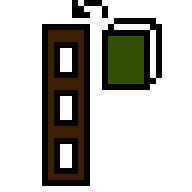
\includegraphics[width=.2\linewidth]{lib_1_1.png}
    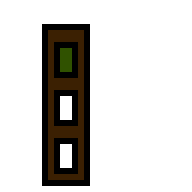
\includegraphics[width=.2\linewidth]{lib_1_2.png}
    \caption{Array als Bücherregal}
    \label{fig:books_arr}
  \end{figure}

  \clearpage

  Wir möchten nun, wie in \ref{fig:books_arr} ein Bücherregal mit drei Fächern erstellen. Dazu
  benötigen wir zuerst eine Klasse, die Bücher darstellen soll:

  \begin{figure}[h]
    \centering
    \lstinputlisting[style=Java]{codes/Book.java}
    \caption{Klasse Book}
  \end{figure}

  Nun können wir ein Bücherregal erstellen:

  \begin{figure}[h]
    \centering
    \lstinputlisting[style=Java]{codes/Book_Array.java}
    \caption{Bücherregal als Array}
    \label{fig:Book_Array}
  \end{figure}

  \clearpage

  Da wir aus der Abbildung \ref{fig:Book_Array} wissen, welche Bücher das Array enthalten soll,
  könnten wir als Alternative auch die Kurzform verwenden:

  \begin{figure}[h]
    \centering
    \lstinputlisting[style=Java]{codes/Book_Array_Shortform.java}
    \caption{Bücherregal als Array - Kurzform}
  \end{figure}


  Natürlich kann der Komponententyp eines Array ebenfalls wieder ein Array sein und man kann
  Arrays auch weiter beliebig viel verschachteln. Damit wäre ein zweidimensionales Array
  (Datentyp[][]) ein Array, wessen Komponententyp eindimensionale Array sind. Bei einem
  dreidimensionalen Array (Datentyp[][][]) sind die Komponententyp zweidimensionale Arrays und
  deren Komponententyp sind jeweils eindimensionale Arrays.

  \begin{note}[title=Information:]
    Beachten Sie, dass die Größe der Arrays innerhalb der Komponenten nicht unbedingt alle gleich
    sein müssen!
  \end{note}

  \br

  Nehmen wir uns als Beispiel wieder das Bücherregal. Wenn wir ein zweidimensionales Array
  betrachten, hat das Bücherregal wieder eine feste Anzahl an Fächern. Diese Anzahl wird vom
  äußeren Array bestimmt. Nun können wir aber die Größe der einzelnen Fächer variieren. Dadurch
  kann beispielsweise das erste Fach maximal ein Buch enthalten, das zweite Fach aber zwei Bücher
  etc.


  \begin{figure}[h]
    \centering
    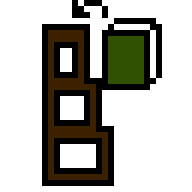
\includegraphics[width=.2\linewidth]{lib_2_1.png}
    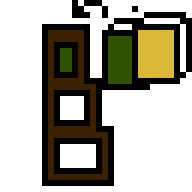
\includegraphics[width=.2\linewidth]{lib_2_2.png}
    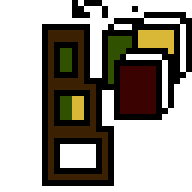
\includegraphics[width=.2\linewidth]{lib_2_3.png}
    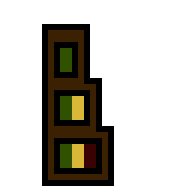
\includegraphics[width=.2\linewidth]{lib_2_4.png}
    \caption{Verschachteltes Array als Bücherregal}
  \end{figure}

  Als Code könnte wir uns das folgendermaßen vorstellen:

  \begin{figure}[h]
    \centering
    \lstinputlisting[style=Java]{codes/Book_Array_Nested.java}
    \caption{Bücherregal als verschachteltes Array}
  \end{figure}

  Da wir auch hier im vorhinein wissen, welche Bücher im Array gespeichert werden sollen, können
  wir wieder die Kurzform verwenden:

  \begin{figure}[h]
    \centering
    \lstinputlisting[style=Java]{codes/Book_Array_Nested_Shortform.java}
    \caption{Bücherregal als verschachteltes Array - Kurzform}
  \end{figure}


  \begin{note}[title=Information:]
    \index{Speicher}
    \index{Speicheradresse}
    Intern im Speicher bezieht sich die Adresse bei einem Array auf die Speicheradresse des
    ersten Elements (Basisadresse). Die nachfolgenden Elemente können von der Basisadresse
    addiert mit einem Offset angesprochen werden. Dieser Offset entspricht der Speichergröße des
    Komponententyps.
    \br
    Beispielsweise um das dritte Element eines Arrays anzusprechen, verwenden wir:

    \begin{center}
      Basisadresse + 2 \(\cdot\) Offset
    \end{center}

    (Die Basisadresse entspricht dem ersten Element. Wenn wir einmal den Offset zu der
    Basisadresse addieren, bekommen wir das zweite Element. Dementsprechend bekommen wir das
    dritte Element, wenn wir zwei Mal den Offset zu der Basisadresse addieren.)

    \br

    Zur Veranschaulichung ist in der folgenden Abbildung ein Array dargestellt, wie es im
    Speicher aussehen würde.

    \begin{figure}[H]
      \centering
      \begin{memory}
        \allocatedummy{5}
        \allocatedummy{15}
        \allocatedummy{25}
        \allocate{8}{12}
        \allocate{18}{18}
        \assign{23}{18}{\inlinejava{a}}
        \assign{2}{8}{\inlinejava{a[0]}}
        \assign{5}{9}{\inlinejava{a[1]}}
        \assign{8}{10}{\inlinejava{a[2]}}
        \assign{14}{11}{\inlinejava{a[3]}}
        \assign{16}{12}{\inlinejava{a[4]}}
        \assignblock{18}{8}
      \end{memory}
      \caption{Abstrakte Visualisierung des Speicherplatzes eines Arrays \inlinejava{a}}
    \end{figure}
    \index{Speicher}

    Wie wir sehen können, verweist \inlinejava{a} auf die Basisadresse, also die Adresse des
    ersten Elements im Array.
  \end{note}

  \clearpage


  \section{Enums}
  \index{Enum}
  \index{Enumeration}
  \index{Klassen}
  \index{Konstanten}
  Enum ist die Kurzform von Ennumeration, was auf deutsch Aufzählung heißt. Enum sind Klassen,
  die von der Klasse
  \href{https://docs.oracle.com/en/java/javase/11/docs/api/java.base/java/lang/Enum.html}
  {java.lang.Enum} abgeleitet sind, und auch Referenztypen. Die Klasse
  \href{https://docs.oracle.com/en/java/javase/11/docs/api/java.base/java/lang/Enum.html}
  {java.lang.Enum} bietet die Möglichkeit, vordefinierte Konstanten für Variablen festzulegen.
  Das ist besonders sinnvoll, wenn die Variablen eine bestimmte und feste Anzahl an Zuständen haben.

  \br

  Wir wollen uns als Beispiel für Enums die Jahreszeiten anschauen, da es nur vier Jahreszeiten
  gibt, die alle einen festen und vordefinierten Namen haben. Wir definieren also ein Enum namens
  \inlinejava{Season}:
  \index{Jahreszeiten}
  \index{Season}

  \begin{figure}[h]
    \centering
    \lstinputlisting[style=Java]{codes/Season.java}
    \caption{Jahreszeiten - Enum Season}
  \end{figure}

  Wenn wir in unserem Programm beispielsweise eine Anweisung ausführen wollen, die nur im
  Frühling stattfinden soll, können wir das folgende Schema verwenden um auf den entsprechenden
  Wert des Enums zuzugreifen:

  \begin{center}
    Season.SPRING
  \end{center}

  Im Allgemeinen lautet also das Schema:

  \begin{center}
    Enumname.Konstantenname
  \end{center}

  Im Speicher kann man sich Enums folgendermaßen vorstellen:

  \begin{figure}[h]
    \centering
    \begin{memory}
      \allocatedummy{5}
      \allocatedummy{15}
      \allocatedummy{25}
      \allocate{8}{11}
      \allocate{18}{18}
      \allocate{20}{20}
      \allocate{22}{22}
      \allocate{27}{27}
      \assign{2}{8}{\inlinejava{SPRING}}
      \assign{5}{9}{\inlinejava{SUMMER}}
      \assign{8}{10}{\inlinejava{AUTUMN}}
      \assign{15}{11}{\inlinejava{WINTER}}
      \assignblock{8}{18}
      \assignblock{9}{20}
      \assignblock{10}{22}
      \assignblock{11}{27}
    \end{memory}
    \caption{Abstrakte Visualisierung des Speicherplatzes des Enums Season}
  \end{figure}
  \index{Speicher}

  Wie wir sehen können, wird ein Enum intern als eine Art Array gespeichert. Wir können dann über
  den Namen der Konstanten auf den jeweiligen gespeicherten Wert zugreifen.

  \printindex
\end{document}
